\documentclass[11pt]{article}
\setlength\parindent{24pt}
\usepackage{indentfirst}
\usepackage[utf8]{inputenc}
\usepackage{subfig}
\usepackage[spanish]{babel}
\usepackage{graphicx}
\usepackage{setspace}		% para doublespacing 
\usepackage{hyperref}		% para hipervinculos
\usepackage[none]{hyphenat}		% para evitar hyphenation
\usepackage{amsmath} % para centrar las ecuaciones 
\numberwithin{equation}{subsection}
\usepackage[section]{placeins}  % para que LaTeX no ponga los floats(imágenes) fuera de sección

\begin{document}

	%\begin{titlepage}
	\begin{center}
		
\includegraphics[scale=0.20]{img/escudoUNC.eps}\\[1cm]
		\textsc{\LARGE Universidad Nacional de C\'{o}rdoba}\\[0.5cm]
		\textsc{\Large Facultad de Matem\'{a}tica, Astronom\'{i}a y F\'{i}sica}\\[2.5cm]
	
		% central heading
			{\doublespacing \LARGE \bfseries
				Reconocimiento de caracteres en im\'{a}genes no estructuradas
			} \\[2.5cm]

			
		% authors and director
		\begin{minipage}{0.4\textwidth}
			\begin{flushleft} \large
				\emph{Autor:}\\
					Rodrigo Carranza Astrada
			\end{flushleft}
			\end{minipage}
			\begin{minipage}{0.4\textwidth}
				\begin{flushright} \large
					\emph{Directores:} \\
						Dr. Jorge Sanchez\\
						Dr. Franco Luque
				\end{flushright}
		\end{minipage}\\[2cm]

		\begin{center}
			\includegraphics[scale=0.7]{./img/license/creative_commons_license.png}
		\end{center}
			Reconocimiento de caracteres en imágenes no estructuradas por Rodrigo Pablo Carranza Astrada se distribuye bajo una \\
			\href{http://creativecommons.org/licenses/by/2.5/ar/}{Licencia Creative Commons Atribución 2.5 Argentina}
			\vfill
	\end{center}
\end{titlepage}


	%\newpage
\section*{Agradecimientos}

	\begin{minipage}{0.9\textwidth}
	Al Dr. Jorge Sanchez y al Dr. Franco Luque, mis directores, por su paciencia, predisposición y ayuda.\\
	A todas las autoridades de FaMAF, sin las que mis aspiraciones académicas y de investigación no hubieran podido concretarse.	\\
	A Juan Norris, amigo y compañero desde el inicio de la carrera, que me ayudo durante la investigación. \\
    A mis padres y hermanos que siempre me apoyaron desde que ingrese a la carrera.
	\end{minipage}

	
	\newpage  % 
	\newpage  % dejamos estas páginas en blanco a propósito
	
	\tableofcontents{}
    \listoffigures{}
    %\listoftables{}
    
	\newpage
\begin{abstract}
	
	\begin{normalsize}

	En esta tesis se presenta un análisis del impacto producido en la performance de clasificación al entrenar un clasificador de caracteres con imágenes sintéticas (Wang et al., 2011). El objetivo es clasificar caracteres en escenas naturales en donde las técnicas tradicinales de OCR no se pueden aplicar de forma directa (De Campos et al., 2009). Para realizar esto, se modifican imágenes de fuentes a través de diferentes transformaciones con el objetivo de simular las condiciones de las imágenes reales. Se complementa este análisis realizando una análisis de performance utilizando diferentes conjuntos de entrenamiento sintéticos generados a partir del dataset público conocido como \textit{Chars74k}. El resultado final de este trabajo sirve para corrobar que la generación de datos sintéticos produce un impacto positivo en la clasificación y más aún si estos se combinan con datos reales.

		{\bf Keywords:} computer vision, Random Ferns, classification, supervised algorithm.

	\end{normalsize}

\end{abstract}
	
	\newpage
	\newpage
\section{Introducción}

	Desde la aparición de las primeras fotografías, las personas han buscado ``inmortalizar'' escenas, objetos o personas, con el objetivo de, en el área de las ciencias, extraer información útil de las mismas que pueda ser utilizada para su análisis o estudio. Con el surgimiento de los primeros formatos digitales, la necesidad pasó por encontrar métodos automáticos que permitieran clasificar y reconocer elementos dentro de las imágenes. Desde reconocer texto manuscrito, texto en carteles publicitarios, patentes, personas, animales, hasta identificar zonas con agua en una imagen satelital. La cantidad de potenciales aplicaciones que se pueden obtener es enorme. Es por eso que en campos de investigación como visión por computadora, este es un tema de interés. Sin embargo, la clasificación en imágenes naturales no es una tarea para nada sencilla. Por ejemplo, en el reconocimiento de texto, las imágenes naturales contienen mucha información ``extra'' que se tiene que tener en cuenta. Ya sea la existencia de otros objetos ajenos a la clasificación, es decir, elementos que no son texto como así también variaciones propias en las características de la misma imagen.
	
	Hoy en día se ha avanzado mucho en el área de la clasificación en escenas naturales. Se han desarrollado muchas aplicaciones como aquellas capaces de reconocer personas \cite{DT05}, hasta las que pueden identificar patentes \cite{DAB}. Si bien, dichos avances muestran que es posible realizar lo mismo en diferentes ámbitos, en otros como el reconocimiento de texto sigue siendo un desafío.
	
	\subsection{El problema}

	La gran cantidad de imágenes y documentos existentes en la actualidad ha motivado el desarrollo de modelos y métodos robustos para la búsqueda automatizada de información con el objeto de reducir los problemas asociados a su análisis e interpretación. La extracción y reconocimiento de texto en imágenes naturales, es decir, imágenes de escenas de la vida diaria y/o adquiridas en condiciones no controladas, es un problema de gran interés, tanto desde el punto de vista teórico como del de las aplicaciones.  Sin embargo, a diferencia del problema de reconocimiento de texto en documentos escaneados, el reconocimiento de texto en imágenes naturales plantea problemas difíciles de abordar mediante el uso de técnicas tradicionales basadas en OCR (\textit{Optical Character Recognition}, por su denominación en inglés). Esto resulta evidente si se consideran los cambios en la iluminación, los distintos puntos de vista, las diferentes tipografías, estilos, objetos que estén en la imagen y generen oclusión en el texto, etc. que se ven reflejadas en imágenes de la vida diaria.

	Una de los esquemas de procesamiento más utilizados ha sido la detección de regiones dentro la imagen que corresponden a texto, su rectificación y la posterior aplicación de técnicas estándar de OCR (Kumar et al., 2007). Sin embargo, esta clase de técnicas se encuentra limitada a los escenarios en donde el OCR funciona correctamente, p.ej. en el reconocimiento de texto impreso (De Campos et al., 2009).

	Recientemente, se propuso un modelo (Wang et al., 2011) que emplea un esquema basado en técnicas de reconocimiento conocidas en la literatura de \textit{reconocimiento de objetos} (Navneet Dalal et al., 2005). En este caso, cada letra del alfabeto se considera como un objeto a detectar y, empleando un conjunto de muestras de entrenamiento, se genera un modelo de clasificación mediante técnicas de aprendizaje supervisado (Christopher M. Bishop, 2007). Dada una nueva imagen, cada uno de estos clasificadores genera un conjunto de hipótesis sobre la presencia (y su ubicación) de cada símbolo alfanumérico en particular. Estas detecciones se utilizan luego en la detección de palabras específicas a partir de un léxico predefinido. Una particularidad del modelo propuesto por Wang et. al es la utilización de imágenes \textit{sintéticas} (generadas mediante simulación) en la generación de muestras de entrenamiento. Este enfoque reduce el problema de tener que recolectar una gran cantidad de imágenes naturales lo cual consume tiempo y esfuerzo. Mediante diferentes tipos de transformaciones, se busca crear un conjunto de caracteres lo más parecido posible a uno real.
	
	
	\subsection{Sobre el trabajo}

	Esta tesis presenta una reimplementación de una sección del trabajo presentado por Wang et. al. en \cite{wang}. En dicha sección, los autores buscan establecer un método para poder reconocer caracteres en imágenes naturales. Para esto proponen usar un clasificador llamado \textit{Random Ferns} (se explica en detalle en el próximo capítulo) para lograr este objetivo.
	
	Este trabajo tiene como finalidad analizar la performance en el reconocimiento de caracteres en imágenes naturales de dicho clasificador. Esto se realiza a través de diferentes experimentos que buscan evaluar diferentes conjuntos de imágenes. El primero es usando imágenes reales, de la misma manera que Wang et. al., con lo cual se busca comparar ambas implementaciones. Posteriormente, se busca analizar como influyen los caracteres sintéticos o fuentes en diferentes proporciones. Estas se alteran con el objetivo de intentar imitar a las imágenes reales y ver si se puede alcanzar o superar los resultados del primer conjunto. Por último y a diferencia de los autores originales, se propone entrenar al clasificador con  un conjunto nuevo que surge de mezclar en diferentes proporciones imágenes reales y sintéticas.

	\subsection{Trabajos Relacionados}
	
	Se han propuesto muchos enfoques para afrontar el problema del reconocimiento de texto en imágenes naturales. De Campos et al. en \cite{dCBV09} comparan la performance de varios clasificadores (dentro de los cuales hay un motor de OCR comercial\footnote{http://abbyy.com/finereader}) sobre un dataset que ellos mismos crearon llamado \textit{Chars74K}. Sobre este dataset se corren varios experimentos del presente trabajo. Las conclusiones del trabajo destacan la dificultad que tienen los motores de OCR al momento de clasificar caracteres en imágenes naturales. Además, remarcan los beneficios de usar datos sintéticos para el entrenamiento los cuales logran un porcentaje de reconocimiento muy similar al obtenido con imágenes reales. También, realizan experimentos sobre un conjunto de imágenes de caracteres manuscritos. Sin embargo, no logran obtener buenos resultados en comparación con los otros experimentos. 
	
	Otro enfoque lo proponen B. Gatos et al. en \cite{GPP03}. El mismo consiste en una nueva metodología que ayuda a la detección, la segmentación y el reconocimiento automático de texto en imágenes naturales. Básicamente, la metodología consiste en lograr una eficiente binarización de las imágenes naturales. Para esto, dada una imagen natural, generan dos imágenes nuevas a partir de la original. La primera es una representación en escala de grises y la segunda es la versión invertida de la primera. Posteriormente, se les aplican diferentes técnicas para mejorarlas y así obtener la imagen binaria. Luego utilizan una función de decisión para elegir qué imagen contiene información de texto y a dicha imagen se le realiza un post-procesamiento para eliminar el ruido existente y mejorar su calidad. Después se realiza la detección de las áreas que contienen texto para poder utilizar finalmente el motor de OCR. Uno de los problemas que se desprenden de este enfoque es que al depender de un motor de OCR, el procesamiento que se realiza a la imagen tiene que ser muy bueno ya que la mayoría de las imágenes contienen ciertos defectos como una pobre iluminación, falta de foco, entre otros.

	L. Neumann y J. Matas \cite{LNJM} se diferencian de los enfoques tradicionales que constan en varias etapas de procesamiento y lo reemplazan con un marco de trabajo que consta de la verificación de hipótesis procesando de manera simultánea múltiples líneas de texto. Además, usan fuente de computadora como conjunto de entrenamiento. Una particularidad de este enfoque es que no se alteran de ninguna manera las fuentes.
	
	
	\subsection{Estructura de la Tesis}

	Esta tesis se desarrolla a lo largo de 5 capítulos.	
		
	En el capítulo 2 se procede a explicar los conceptos teóricos que involucran el presente trabajo. Principalmente se abordan los principios básicos del aprendizaje supervisado. Posteriormente se describen los conceptos ne\-ce\-sa\-rios para poder introducir  el clasificador Random Ferns. Finalmente, se rea\-li\-za una introducción a las nociones básicas del procesamiento de imágenes.
	
	 En el capítulo 3, se describe el trabajo realizado por Wang et al. en \cite{wang} y se explica qué partes del mismo se han implementado en la presente tesis.

	En el capítulo 4, se abordan los experimentos realizados en el trabajo. Se describe tanto la implemetación del pipeline de procesamiento, como así también su diseño, el dataset usado y los resultados obtenidos. Por último se realiza un análisis completo de los resultados.
	
	En el último capítulo, de conclusiones y trabajos futuros, se hace un resumen de lo logrado a lo largo de esta tesis así como un descripción de los objetivos futuros que se pretenden seguir en este trabajo.

	
	%\subsection{Sobre Reconocimiento óptico de caracteres}

	\subsubsection{Definición del problema}
	
	El reconocimiento óptico de caracteres, usualmente abreviado OCR(por sus siglas en inglés), es la conversión mecánica o electrónica de imágenes escaneadas de texto impreso o mecanografiado en texto que pueda ser interpretado por una computadora. Es ampliamente utilizado como una forma de entrada de datos de algún tipo de fuente de datos original en papel, así sean documentos de pasaportes, facturas, extractos bancarios, recibos, tarjetas de visita, correo, o cualquier número de registros impresos\cite{arh-passport}\cite{arh-card}. Es un método común para la digitalización de textos impresos que pueden ser electrónicamente editados, buscados, almacenados de manera compacta, expuestos en linea y usados en procesos de máquinas como traducción de máquina, texto a voz, extracción de datos y minería de texto\cite{gbook}\cite{creaceed}. OCR es un campo de investigación en reconocimiento de patrones, inteligencia artificial y visión por computadora.
	
	\subsubsection{Aplicaciones}
		\begin{itemize}
			\item Reconocimiento automático de patentes\cite{arh-anpr}.
			\item Extraer información de una tarjeta de negocio a una lista de contacto \cite{x-root}.
			\item Hacer posible la búsqueda de imágenes electrónicas de documentos impresos. ej: \textit{Google Books} \cite{gbook}
			\item Convertir la escritura manual en tiempo real para controlar una computadora (\textit{pen computing})\cite{GKurt}\cite{sunnyside}.
			\item Tecnología de asistencia para usuarios ciegos y con deficiencias visuales \cite{creaceed}.
		\end{itemize}	
		
	\subsubsection{Componentes de un sistema OCR}
	
	A continuación se presentaran las diferentes etapas de un sistema OCR, como se puede apreciar en la figura \ref{fig: Sistema OCR}. Esta sección tiene como objetivo mostrar un panorama general de como funciona un sistema OCR, no tiene como objetivo adentrarse en detalles de implementación. En cada etapa se procederá a explicar brevemente cuales son las características importantes, haciendo incapié en la etapas de extracción de características y en la de clasificación y reconocimiento dado que son las etapas que se abordaron en este trabajo.
	
		\begin{figure}[htbp]
			\centering
			\fbox{ \includegraphics[scale=0.4]{img/OCR_pipeline_1.jpg} }
			\caption{Pipeline de un sistema OCR.}
			\label{fig: Sistema OCR}
		\end{figure}
	
		\paragraph{Pre-procesamiento} ~\\

		 El software de OCR aveces realiza un pre-procesamiento de las imágenes con el objetivo de tener más chances de un reconocimiento exitoso. Estas técnicas incluyen:
		  \begin{itemize}
		  	\item \textit{Enderezar} - Si el documento no está alineado debidamente cuando se escanea, puede necesitar posteriormente que se rote unos pocos grados en sentido horario o anti-horario con el objetivo de mantener el texto perfectamente vertical u horizontal \ref{fig: Enderezar}.
		  	\item \textit{Quitar manchas} - remover puntos negativos  y positivos, suavizar los bordes \ref{fig: Imagen con particulas} \ref{fig: Imagen suavizada}.
		  	\item \textit{Binarización} - Convertir la imagen de color o en escala de grises a blanco y negro (se llama "imagen binaria" justamente porque hay dos colores solamente). En algunos casos, esto es necesario para el algoritmo de reconocimiento de caracteres; en otros casos esta etapa se omite dado que el algoritmo tiene un mejor rendimiento con la imagen original \ref{fig: Binarizacion}.
		  	\item \textit{Eliminación de lineas} - Limpia las lineas y las cajas sin glifo \ref{fig: Eliminacion de lineas}.
		  	\item \textit{Análisis de disposición o "zoning"} - Identifica columnas, párrafos, títulos, etc. como bloques diferentes. Especialmente importante en tablas o disposiciones multi-columna \ref{fig: Zoning}.
		  	\item \textit{Detección de lineas y palabras} - Establece  la base para la forma del caracter y la palabra, separa las palabras si es necesario.
		  	\item \textit{Segmentación o aislación de caracter} - Múltiples caracteres que están conectados debido a artefactos de imagen deben ser separados; caracteres individuales que son separados en multiples piezas debido a artefactos deben ser conectados \ref{fig: Segmentacion}.
		  	\item \textit{Normalización de escala y relación de aspecto \ref{fig: Normalizacion y Suavizado}.}
		  \end{itemize}
		  
		\begin{figure}[htbp]
			\centering
			\subfloat[Imagen original torcida\label{fig: Imagen torcida}]{
				\fbox{ \includegraphics[scale=0.7]{img/skew_img.png} }
			}
			\subfloat[Imagen enderezada\label{fig: Imagen destorcida}]{
				\fbox{ \includegraphics[scale=0.7]{img/deskew_img.png} }
			}
			\caption{Imagen enderezada}
			\label{fig: Enderezar}
		\end{figure}	
			  
		\begin{figure}[htbp]
			\centering
			\fbox{ \includegraphics[scale=0.4]{img/rem_particles.png} }
			\caption[Imagen con partículas]{Comparación de caracteres con y sin partículas. 1. Imagen con partículas.}
			\label{fig: Imagen con particulas}
		\end{figure}
		
		\begin{figure}[htbp]
			\centering
			\fbox{ \includegraphics[scale=0.4]{img/smooth_char.png} }
			\caption{Imagen suavizada.}
			\label{fig: Imagen suavizada}
		\end{figure}
		
		\begin{figure}[htbp]
			\centering
			\subfloat[Imagen Original\label{fig: Imagen bin original}]{
				\fbox{ \includegraphics[scale=0.7]{img/bin_1.png} }
			}
			\subfloat[Imagen binarizada\label{fig: Imagen binarizada}]{
				\fbox{ \includegraphics[scale=0.7]{img/bin_2.png} }
			}
			\caption{Binarización de una imagen}
			\label{fig: Binarizacion}
		\end{figure}
		
		\begin{figure}[htbp]
			\centering
			\subfloat[Imagen Original\label{fig: Imagen lines original}]{
				\fbox{ \includegraphics[scale=0.7]{img/lines_1.png} }
			}
			\subfloat[Imagen con las lineas removidas\label{fig: Imagen sin lineas}]{
				\fbox{ \includegraphics[scale=0.7]{img/lines_2.png} }
			}
			\caption{Eliminación de lineas}
			\label{fig: Eliminacion de lineas}
		\end{figure}
		
		\begin{figure}[htbp]
			\centering
			\fbox{ \includegraphics[scale=0.3]{img/zoning.png} }
			\caption{Análisis de disposición o "zoning".}
			\label{fig: Zoning}
		\end{figure}

		\begin{figure}[htbp]
			\centering
			\fbox{ \includegraphics[scale=0.5]{img/segmentation.png} }
			\caption[Segmentación]{Segmentación. 1.Imagen Adquirida, 2.Región de interés, 3.Rectángulo del límite del carácter, 4.Carácter, 5.Artefacto, 6.Elemento, 7.Espaciado vertical, 8.Espaciado horizontal, 9.Espaciado del carácter.}
			\label{fig: Segmentacion}
		\end{figure}
		
		\begin{figure}[htbp]
			\centering
			\fbox{ \includegraphics[scale=0.4]{img/norm_and_smoothing.png} }
			\caption{Normalización y suavizado de un símbolo.}
			\label{fig: Normalizacion y Suavizado}
		\end{figure}
	
\newpage
		\paragraph{Ubicación y segmentación}	 ~\\
		
		La segmentación es el proceso que determina los componentes de una imagen. Es necesario ubicar las regiones del documento donde se han impreso los datos y distinguirlos de los gráficos y las figuras. Por ejemplo, cuando se realiza el ordenamiento de correo automático, la dirección debe estar localizada y separada de otras impresiones en el sobre como las estampillas o logos de empresa, anterior al reconocimiento.
		
		Aplicado al texto, la segmentación es la aislación de caracteres o palabras. La mayoría de los algoritmos de reconocimiento óptico de caracteres segmentan las palabras en caracteres aislados los cuales son reconocidos individualmente. Usualmente esta segmentación es realizada aislando cada componente conectado, es decir, cada área negra conectada. Esta técnica es fácil de aplicar, pero los problemas ocurren si los caracteres se tocan o si los caracteres están fragmentados y consisten de varias partes, si el texto tiene mucho ruido o se confunde con alguna imagen, entre otros. ~\ref{fig: Caracter quebrado}~\ref{fig: Caracteres unidos 1}~\ref{fig: Caracteres unidos 2}~\ref{fig: Caracteres en graffiti}~\ref{fig: Captcha}.

		\begin{figure}[htbp]
			\begin{minipage}{.3\linewidth}
				\centering
				\subfloat[Captcha\label{fig: Captcha}]{
					\fbox{ \includegraphics[scale=0.2]{img/degraded_1.jpg} }
				}
			\end{minipage}
			\begin{minipage}{.3\linewidth}
				\centering
				\subfloat[Carácter quebrado\label{fig: Caracter quebrado}]{
					\fbox{ \includegraphics[scale=0.3]{img/degraded_2.jpg} }
				}
			\end{minipage}
			\begin{minipage}{.3\linewidth}
				\centering
				\subfloat[Caracteres unidos por la tipografía\label{fig: Caracteres unidos 1}]{
					\fbox{ \includegraphics[scale=0.3]{img/degraded_3.jpg} }
				}
			\end{minipage}
			\begin{minipage}{.3\linewidth}
				\centering
				\subfloat[Carácter con linea superpuesta\label{fig: Caracter y linea}]{
					\fbox{ \includegraphics[scale=0.3]{img/degraded_4.jpg} }
				}
			\end{minipage}
			\begin{minipage}{.3\linewidth}
				\centering
				\subfloat[Caracteres unidos\label{fig: Caracteres unidos 2}]{
					\fbox{ \includegraphics[scale=0.3]{img/degraded_5.jpg} }
				}
			\end{minipage}
			\begin{minipage}{.3\linewidth}
				\centering
				\subfloat[Un graffiti como el de la imagen puede hacer pasar el texto como imagen.\label{fig: Caracteres en graffiti}]{
					\fbox{ \includegraphics[scale=0.2]{img/text_like_graphic.jpg} }
				}
			\end{minipage}
			\caption{Problemas de segmentación}
			\label{fig: Problemas de segmentacion}
		\end{figure}
		
	
		\paragraph{Extracción de características} ~\\
		
		El objetivo de la extracción de características es capturar los rasgos esenciales de los caracteres para formar vectores de características y es generalmente aceptado como uno de los problemas más difíciles en el reconocimiento de patrones. Se vuelve sencillo para el clasificador el clasificar entre clases diferentes teniendo en cuenta estas características \cite{PSH2011}. Acorde al trabajo de C. Y. Suen \cite{Suen86}, los rasgos de un carácter pueden ser clasificados en dos clases: características globales o estadísticas y características estructurales o topológicas.
		\begin{itemize}
			\item \textbf{Características globales o estadísticas}. \\
				Las características globales son obtenidas del arreglo de puntos que constituyen la matriz del carácter. Estas características pueden ser detectadas fácilmente en comparación con las características topológicas. Además no son afectadas demasiado por el ruido o la distorción en comparación a las topológicas. Un número de técnicas se utilizan para lograr la extración de características, estas son: \textit{momentos, zonificación, histogramas de proyección, n-tuplas y cruce y distancias}
				\begin{itemize}
					\item \textbf{Momentos}
					En este caso los diferentes puntos presentes en un carácter son utilizados como características. Heutte et al. \cite{Heutte98} decían que estos métodos son más comúnmente usados en el reconocimiento de caracteres.
					\item \textbf{Zonificación}
					De acuerdo con esta técnica, la matriz del carácter es dividida en pequeñas porciones o zonas. Las densidades de los píxeles en cada zona son calculadas y usadas como características. Este concepto fue sugerido por Hussain et al.\cite{Hussain72}.
					\item \textbf{Histogramas de proyección}
					Los histogramas de proyección nos da el número de píxeles negros en las direcciones horizontal y vertical de un área específica del carácter. El concepto fue introducido por M. H. Glauberman \cite{Glauberman56}. Los histogramas de proyección pueden ser vertical, horizontal, diagonal izquierda o derecha.
					\item \textbf{N-tuplas}
					De acuerdo con este método, la posición de los píxeles blancos o negros en la imagen de un carácter es considerado una característica. El método fue desarrollado por Tarling y Rohwer \cite{TR93}.
				\end{itemize}
			\item \textbf{Características estructurales o topológicas}. \\
				Estas características están relacionadas con la geometría del conjunto de caracteres. Algunas de estas características son concavidades y convexidades en los caracteres, el número de puntos finales, el número de agujeros en los caracteres, etc. Muchas investigaciones fueron realizadas con el objetivo de encontrar diferentes características estructurales.
				
				Rocha y Pavlidis \cite{RP94} propusieron un método para el reconocimiento de caracteres impresos del tipo multi-fuente. Para este método se han utilizado características estructurales tales como puntos singulares, arcos convexos y trazos.
				
				Otro método similar fue propuesto por A. Amin \cite{Amin2000}. Aquí se han usado características estructurales como el número de subpalabras, el número de picos en cada subpalabra, el número de curvas de cada pico, entre otros.
				
		\end{itemize}
		  
		  	En el presente trabajo, las características de una imagen son representadas por un vector binario que se obtiene de binarizar el descriptor HOG(concepto descripto en la sección \ref{sec: HOG}) de dicha imagen con un umbral pre-calculado. Este método de extracción de características se abordará más adelante en el capítulo 4 cuando se explique el pipeline de procesamiento.
	  
		\paragraph{Clasificación y Reconocimiento} ~\\
		
		La clasificación es el proceso de identificar cada carácter y asignarle la clase correcta. La clasificación se hace generalmente mediante la comparación de los vectores de características que corresponden al carácter de entrada con el representante de cada clase de carácter. Pero antes de hacer esto, el clasificador debe entrenarse con un conjunto de entrenamiento que represente a las diferentes clases de caracteres. Varios investigadores han propuesto métodos de clasificación dentro de los cuales se encuentran los métodos estadísticos, métodos sintácticos, comparación de plantillas, redes neuronales artificiales, métodos de núcleo~\cite{NNSJ}~\cite{SA96}~\cite{RYVY2010}.
		
		Como se procederá a explicar en detalle en el capítulo 3, el clasificador que se usa en este trabajo es Random Ferns. Las razones de su elección se basan en que es un clasificador multi-clase bastante eficiente y dado que el problema en cuestión es clasificar caracteres (representan 62 clases en total), su elección resulta apropiada.
		
		El aporte de este trabajo se basa en analizar la performance del clasificador Random Ferns cuando es entrenado con caracteres sintéticos. Si bien este enfoque fue abordado en \cite{wang}, en dicho trabajo no se puede apreciar como influye en la clasificación la cantidad de imágenes sintéticas usadas al entrenar el clasificador. En su trabajo, hacen uso de 1000 imágenes sintéticas por clase para entrenar el clasificador y realizan una comparación de performance entre el entrenamiento con imágenes sintéticas y el realizado con imágenes reales. Este trabajo va un paso más allá y busca ver si el número de imágenes sintéticas por clase influye realmente en la performance y además se busca analizar un nuevo enfoque en el cual se mezclan en diferentes proporciones imágenes reales con sintéticas para observar que tan efectivo resulta ser el clasificador en esas condiciones.
		
		\paragraph{Post-procesamiento} ~\\
		
		La precisión de OCR puede ser incrementada si la salida está restringida por un lexicón, que es una lista de palabras cuya aparición está permitida dentro del documento. Este puede ser, por ejemplo, todas las palabras del lenguaje español, o un lexicón mas técnico para un campo en particular. Esta técnica puede ser problematica si el documento contiene palabras que no están en el lexicón, como nombres propios.
		
		La salida puede ser texto plano o un archivo de caracteres, pero sistemas de OCR más sofisticados pueden conservar la disposición original de la pagina y producir, por ejemplo, un PDF con anotaciones que incluyan la imagen original de la página y una representación textual de búsqueda.
		
		Conocer la gramática del lenguaje que está siendo escaneado puede ayudar a determinar si la palabra es un verbo o un sustantivo, por ejemplo, permitiendo una gran precisión.
		
	\subsubsection{Errores típicos en OCR}
	
		La precisión de los sistemas de OCR es, en la práctica, directamente dependiente de la calidad de los documentos de entrada. Las principales dificultades se pueden clasificar como sigue:
		\begin{itemize}
			\item \textit{Variaciones en la forma}, debido a las variaciones en el estilo y los remates o serifas.
			\item \textit{Deformaciones}, causados por caracteres quebrados, manchados y moteados.
			\item \textit{Variación en el espaciado}, debido a los superíndices, subíndices, sesgo y la variable de espaciado.
			\item \textit{Mezcla de texto e imágenes}.
		\end{itemize}
		Estas imperfeccciones pueden afectar y ocasionar problemas las diferentes etapas del proceso de reconocimiento de un sistema OCR, resultando en errores de clasificación y rechazos.	
	
		

	
	%	\newpage
	\subsection{Repercusión social del tema}
		\label{sec:repercusion_social}
		Cheap brainstorm:
		\begin{itemize}
		 \item digitalizar documentos
		 \item brindar mejor calidad de  vida a gente con discapacidades
		 
		\end{itemize}



	
	\newpage	
\section{Marco teórico}

	\subsection{Aprendizaje automático}

	Desde la máquina construida por Blaise Pascal en 1642 para realizar sumas, la primera computadora programable electrónica ENIAC hasta la actualidad, el hombre siempre ha demostrado interés por automatizar ciertos procesos. En particular, el tener una máquina que pudiera leer como una persona era un sueño, que tuvo sus inicios alrededor de 1914 cuando Edmund Fournier d'Albe desarrolló el \textit{Optophone} (ver figura \ref{fig: Optophone}), que era un escáner de mano que al moverlo a través de una página impresa, producía tonos que correspondían	a letras o caracteres específicos \cite{EFdAlbe}.

			\begin{figure}[htbp]
				\centering
				\centerline{
					\includegraphics[scale=1]{img/Optophone.jpg}
				}
				\caption[Optophone]{Imagen del \textit{Optophone} en detalle. Extraida de la revista Vetenskapen och livet (1922).}
				\label{fig: Optophone}
			\end{figure}
			
	Durante gran parte del siglo \rom{20} y hasta el día de hoy, la cantidad de información almacenada en libros y documentos escritos ha crecido de manera exponencial. Esto se debe a que cada día se vive en un mundo más globalizado, donde la información es una herramienta fundamental en cualquier ámbito. Con el surgimiento de las primeras computadoras y la digitalización de la información, se volvió más fácil compartir datos. Sin embargo, el proceso de digitalizar los documentos ya existentes era un proceso tedioso ya que se hacía manualmente. Debido a esto, era imperativo tener algún método automático que ayudara a clasificar y analizar toda esa información ya que sobrepasaba la capacidad de las personas de hacerlo por sí mismas. Dada esta necesidad es que surge el campo de \textit{aprendizaje automático} o \textit{machine learning} para proveer métodos que resuelvan estos problemas. El aprendizaje automático estudia métodos que permiten detectar automáticamente patrones en los datos y luego usar esos patrones descubiertos para predecir datos futuros o poder tomar ciertas decisiones en condiciones de incertidumbre. 
	
	Uno de los temas que se tratan en este campo es el del reconocimiento de texto en imágenes. Las aplicaciones son muy numerosas, desde ayudar a las personas no videntes \cite{Optelec}, realizar detección de patentes \cite{DAB} o hacer traducción automática de textos en diferentes idiomas \cite{WordLens}.
	 
	 El campo de \textit{machine learning} tiene fuertes bases en la estadística por lo cual, conceptos como los desarrollados en el apéndice \ref{section:Apendice-A} sobre ``Conceptos de probabilidad y notación'' van a ser de utilidad para comprender las siguientes subsecciones.
	 
	 De todas las áreas existentes en este campo, las más destacadas e importantes son las de: aprendizaje supervisado y no supervisado. Las mismas se van a ver a continuación.
	 	
	\subsubsection{Aprendizaje supervisado}
	
	El aprendizaje supervisado es una rama del aprendizaje automático cuyo objetivo es, dado un conjunto de entradas denotado por $X$ y uno de salidas denotado por $Y$, establecer un mapeo entre $X$ e $Y$ dado un conjunto etiquetado de pares de entrada-salida $M=\{(x_i,y_i) x_i \in X, y_i \in Y \}^{N}_{i=1}$ donde $M$ es llamado el \textit{conjunto de entrenamiento} y $N$ es el número de ejemplos de entrenamiento.
	
	El conjunto de entrenamiento es un elemento indispensable en cualquier algoritmo de aprendizaje supervisado, ya que representa la base fundamental de conocimiento necesaria para que algoritmo pueda realizar futuras predicciones. En general, mientras más conocimiento se tenga sobre las características del objeto de interés que se esté analizando, más precisa va a ser la clasificación sobre nuevas entradas. Esto último hace referencia al concepto de \textit{generalización}, es decir, la habilidad de interpretar con precisión nuevas entradas luego de haber ``experimentado'' un conjunto de entrenamiento. Este conocimiento se construye a partir de la variabilidad de los objetos conocidos, es decir el poder contar con un gran conjunto de muestras que reflejen las posibles variaciones del objeto de interés. Esto le otorga robustez a la clasificación. 
	
	En la configuración más simple, cada entrada $x_i$ del conjunto de entrenamiento es un vector $D$-dimensional de números. Estas son llamadas \textit{características} (\textit{features}, de su traducción al inglés). En general, sin embargo, $x_i$ puede ser un objeto con una estructura compleja, como una imagen, un mensaje de correo, etc.
	
	Dependiendo del tipo de problema a tratar, la salida $y_i$ puede ser una variable categórica, donde $y_i \in \{1,\dots,C\}$ (conjunto finito de clases), o puede ser un valor real. Cuando $y_i$ es una variable categórica, estamos frente a un problema de \textit{clasificación} donde el objetivo es ``etiquetar'' o nombrar los objetos observados. Cuando $y_i$ es una variable real, estamos en presencia de un problema de regresión, que es similar a la clasificación excepto que la respuesta es en general una variable continua.
	
	Por ejemplo, consideremos un clasificador de caracteres alfanuméricos que tiene como conjunto de entrenamiento un grupo de imágenes que representan a cada carácter individualmente. Luego, dado que un carácter puede estar representado de diferentes formas, es decir, pueden haber variaciones en la perspectiva del mismo, en la iluminación del ambiente, el ruido de la imagen, entre otros, es necesario poder contar con la mayor cantidad de estas variaciones. Esto se debe a que mientras más conocimiento se tenga sobre las características del objeto de interés y las diferentes formas en que este puede aparecer, más certera va a ser la clasificación sobre nuevas entradas. Esto es lógico pues las nuevas entradas van a ser variaciones de los elementos que tenemos en el conjunto de entrenamiento. Es importante que el
	

	\subsubsection{Aprendizaje no supervisado}
	
		El aprendizaje no supervisado es la otra rama del aprendizaje automático cuyo objetivo es encontrar ``estructuras interesantes'' en los datos. A diferencia del aprendizaje supervisado, no se establece qué salida se tiene que dar para cada entrada. En cambio, se busca construir modelos de la forma $p(x_i | \theta)$ donde $\theta$ es un vector de parámetros y $x_i$ es un dato de entada. La diferencia con el aprendizaje supervisado, es que hemos establecido $p(x_i | \theta)$ en vez de $p(x_i | y_i, \theta)$; es decir, el aprendizaje supervisado es una estimación condicional en la variable de interés, mientras que el aprendizaje no supervisado es una estimación no condicional.
		
		El aprendizaje no supervisado no requiere de que haya una persona que etiquete los datos manualmente, lo cual no solo es costoso, sino que además contiene relativamente poca información, sin duda no es suficiente para estimar de forma fiable los parámetros en modelos más complejos.
	
	\subsection{Clasificación}

		Como explica de manera sencilla Murphy K. P. en \cite{Murphy12}, el objetivo del aprendizaje supervisado es aprender un mapeo desde las entradas $x$ a las salidas $y$. En clasificación, $y_i \in \{1,\dots,C\}$ con $C$ siendo el número de clases. Si $C=2$, estamos frente al problema de \textit{clasificación binaria}; mientras que si $C>2$, la clasificación pasa a ser \textit{multiclase}. Existe otro tipo de clasificación denominada \textit{clasificación multi-etiqueta}, que difiere de la multiclase en cuanto a que las clases no son mutuamente excluyentes, es decir, una muestra puede pertenecer a dos o más categorías o clases. En este último caso, el mapeo se realiza desde la entrada $x$ a un vector $z$, más que a una salida escalar. La elección de cual usar esta directamente asociada al tipo de problema que se quiera resolver.
		
		Una manera de formalizar el problema es a partir de una función de aproximación. Se asume $y = f_{\theta}(x)$ para cierta función desconocida $f_{\theta}$, y el objetivo del aprendizaje es estimar los parámetros $\theta$ de la función $f$ dado un conjunto de entrenamiento etiquetado. Posteriormente, se realizan predicciones usando $\hat{y} = f_{\hat{\theta}}(x)$ (usamos el símbolo \string^ para denotar estimación). El objetivo principal es realizar predicciones en entradas nuevas, es decir, que no se hayan visto durante el entrenamiento.
		
		Tal como expresa P. Domingos en \cite{PDomingo} el objetivo del aprendizaje automático es \textit{generalizar} más allá de los ejemplos en el conjunto de entrenamiento. Ya que, no importa cuantos datos tengamos, es muy poco probable que vayamos a ver los mismos ejemplos al momento de evaluar.

	\subsubsection{Clasificadores Probabilísticos}

		Los clasificadores probabilísticos determinan, dada una entrada nueva, la probabilidad de que esta pertenezca a un conjunto de clases, a diferencia de otros clasificadores, que simplemente predicen a que clase pertenece la misma. Esto lo realiza asignando una distribución de probabilidad al conjunto de clases.
	
	Formalmente un clasificador probabilistico es una distribución condicional $p(Y|X)$ sobre un conjunto finito de clases $Y$ dada $X$ entradas. Una forma de determinar cual es la mejor clase $\hat{y} \in Y$ para $X$ sería elegir la clase con la probabildiad más alta
	$$\hat{y} = argmax_{y}p(Y=y|X) $$
	
	Uno de los clasificadores más populares es \textit{na\"{i}ve Bayes} (que se procede a explicar en las proximas secciones). Este clasificador junto con el resto derivan de modelos de probabildiad generativos que proporcionan un principio para el estudio de la clasificación estadística en dominios complejos tales como el lenguaje natural y el procesamiento visual \cite{GargRo01}.


	\subsubsection{Teoría de decisión}
	
	La teoría de decisión nos ayuda a tomar decisiones óptimas en situaciones que involucran incertidumbre. La incertidumbre hace referencia a un estado de conocimiento limitado donde es imposible describir con exactitud el estado existente, la salida futura, o más de una posible salida.
	
	Supongamos que tenemos un vector $x$ como entrada junto con el correspondiente vector $t$ de variables objetivo, la meta es predecir $t$ dado un nuevo valor de $x$. En problemas de regresión, $t$ comprenderá variables continuas, mientras que en problemas de clasificación $t$ representará etiquetas de clase. La determinación de $p(x,t)$ dado un conjunto de datos de entrenamiento es un ejemplo de \textit{inferencia} y es típicamente un problema muy difícil. La inferencia, en este caso, hace relación a la estadística inferencial la cual es una parte de la estadística que comprende los métodos y procedimientos que por medio de la inducción determina propiedades de una población estadística, a partir de una pequeña parte de la misma.
	
	Consideremos el siguiente ejemplo, sea $C=\{C_1,\dots,C_k\}$ un conjunto de etiquetas de clase, sea $t \in C$ y sea $x$ un vector de entrada nuevo. Se desea determinar a que clase pertenece $x$. El problema de inferencia involucra determinar la distribución conjunta $p(x,C_k)$, o equivalentemente $p(x,t)$.

	Como se dijo anteriormente, el objetivo es decidir a cual de las $k$ clases pertence el vector de entrada $x$ . Estamos interesados entonces, en las probabilidades de las $k$ clases dado $x$, es decir $p(C_k|x)$, $k=1,\dots,K$. Usando el Teorema de Bayes, estas probabilidades pueden expresarse de la forma:
		\begin{align*}
			p(C_k|x) = \frac{p(x|C_k)p(C_k)}{p(x)}
		\end{align*}

	Ahora podemos interpretar $p(C_k)$ como la probabilidad a priori para la clase $C_k$, y $p(C_k|x)$ como la correspondiente probabilidad a posteriori. Por ejemplo, $p(C_1)$ representa la probabilidad de pertenecer a la clase $C_1$, antes de observar la muestra $x$
	
	Se pueden distinguir dos etapas en el problema de clasificación, la \textit{etapa de inferencia} en el cual se usan los datos para entrenar el modelo para $p(C_k|x)$, y la subsecuente \textit{etapa de decisión} en la cual se usan las probabilidades a posteriori para poder realizar asignaciones óptimas de las clases. Una alternativa, es la de resolver ambos problemas en conjunto y simplemente entrenar una función que mapee las entradas $x$ directamente con las decisiones. Dicha función es llamada \textit{función discriminante}.
	
	De hecho, se pueden identificar tres enfoques diferentes al momento de resolver problemas de decisión. En orden decreciente de complejidad, estos son:
		\begin{enumerate}
			\item Primero, resolver el problema para determinar las densidades condicionales $p(x \vert C_k)$ para cada clase $C_k$ individualmente. También de forma separada, inferir las probabilidades de clases a priori $p(C_k)$. Después, usar el teorema de Bayes en la forma:
			$$p(C_k \vert x) = \frac{p(x \vert C_k)p(C_k)}{p(x)} $$
			para encontrar las probabilidades a posteriori $p(C_k \vert x)$. Como es usual, el denominador en el teorema de Bayes puede ser encontrado en término de las cantidades que aparecen en el numerador, como:
			 $$p(x) = \sum_k p(x \vert C_k)p(C_k) $$
			Equivalentemente, se puede modelar la distribución conjunta $p(x,C_k)$ directamente y después normalizar para obtener las probabilidades a priori. Habiendo encontrado las probabilidades a posteriori, se puede usar la teoría de decisión para determinar la pertenencia a una clase para cada entrada nueva $x$. Los enfoques que explícitamente o implícitamente modelan la distribución de las entradas así también como las salidas son conocidos como \textit{modelos generativos}, debido a que tomando muestras de ellos es posible generar puntos de datos sintéticos en el espacio de entrada.
			\item Primero, resolver el problema de inferencia para determinar las  probabilidades de clase a posteriori $p(C_k \vert x)$, y luego subsecuentemente usar la teoría de decisión para asignar a cada $x$ nueva una de estas clases. Los enfoques que modelan las probabilidades a posteriori directas son llamados \textit{modelos discriminativos}.
			\item Encontrar una función $f(x)$, llamada función discriminante, que mapea directamente cada entrada $x$ con una etiqueta de clase. Por ejemplo, en el caso del problema de dos clases, $f(\cdot)$ puede ser valuada de manera binaria, de manera que $f = 0$ represente a la clase $C_1$ y $f = 1$ represente a la clase $C_2$. En este caso, las probabilidades no toman partido. 
		\end{enumerate}
		
	Consideremos los méritos relativos a estas tres alternativas. El enfoque (1) es el más demandante debido a que involucra encontrar la distribución conjunta tanto de $x$ como de $C_k$. Para muchas aplicaciones, $x$ tendrá alta dimensionalidad, y por consiguiente puede ser necesario un conjunto de entrenamiento grande con el fin de ser capaz de determinar las densidades de clase condicional con una exactitud razonable. Hay que tener en cuenta que la probabilidades a prior $p(C_k)$ de la clase a menudo pueden estimarse simplemente a partir de las proporciones de los punto de datos del conjunto de entrenamiento en cada una de las clases.
		
	Sin embargo, si sólo deseamos realizar decisiones de clasificación, esto conlleva a un gasto de recursos computacionales y una demanda de datos excesiva para encontrar la distribución conjunta $p(x, C_k)$ cuando de hecho, solamente se necesitan las probabilidades a posteriori $p(C_k \vert x)$, las cuales pueden ser obtenidas a través del enfoque (2). 
		
	Un enfoque mucho más simple es (3) en el cual se usa una conjunto de entrenamiento para encontrar una función discriminante $f(x)$ que mapea cada $x$ directamente a una etiqueta de clase, así combinando la inferencia y las etapas de decisión en un simple problema de aprendizaje.
		
	Con la opción (c), sin embargo, se pierde el acceso a las probabilidades a porteriori $p(C_k \vert x)$. 
	
	\subsubsection{Vectores de características} \label{subsection:feature}
	
	Hasta el momento, se ha introducido la idea general de qué es un clasificador probabilístico. Se detalló que estos clasificadores toman una ``entrada \textit{X}'' y le asignan una probabildiad de que dicha entrada pertenezca a cada una de las clases asociadas. El proceso interno para realizar esto varia entre clasificadores, sin embargo, un concepto necesario para comprender cómo trabajan cuando ``procesan'' una entrada es el de \textit{característica}.

	Una \textit{característica} o \textit{feature}, es un aspecto o cualidad distintiva de un objeto (clase de interés). Las características son importantes dado que al re\-pre\-sen\-tar los aspectos o cualidades más significativas de un objeto, facilitan el reconocimiento posterior de objetos similares \cite{OIVIND95}. Esto es fundamental por ejemplo, en los esquemas de clasificación en el aprendizaje supervisado ya que permite, dada una muestra desconocida, identificar a qué clase pertenece si anteriormente sabemos las características particulares de cada clase (a partir de instancias o muestras analizadas con anterioridad). Esto conlleva a que si se realiza una buena selección de características, impacte positivamente en la precisión de los clasificadores y por ende en el reconocimiento. Por ejemplo, en los algoritmos de detección de spam, las características pueden incluir el lenguaje en el que está escrito el email, la ausencia o presencia de ciertos encabezados, la corrección gramatical del texto, entre otros~\cite{SpamPaper}.

	Un \textit{vector de características} o ``feature vector'' se lo puede definir como un conjunto de características que definen a un objeto. Dicho objeto, en adelante $X$, es representado por un vector $D$-dimensional tal que  $X=(x_1,\dots,x_D)$ donde los $x_i$ representan a las características del objeto. En general, $x_i, i=1,\dots,D$ son numéricas dado que dicha representación facilita el análisis estadístico y el procesamiento de datos.

	En base a lo explicado anteriormente, se presenta a continuación al primer clasificador probabilístico que va a servir de ayuda para comprender los siguientes clasificadores.
		
	

	
	\subsubsection{Clasificador Na\"{i}ve Bayes}

	En \cite{NarasMurty}, Narasimha y Susheela definen a Na\"{i}ve Bayes como un clasificador probabilístico basado en la aplicación del Teorema de Bayes con una fuerte suposición de independencia, na\"{i}ve. En términos simples, los autores detallan que un clasificador Na\"{i}ve Bayes asume que la presencia o ausencia de una característica particular no está relacionada con la presencia o ausencia de cualquier otra característica. Este tipo de clasificador considera que cada una de estas características contribuye independientemente a la probabilidad de que un elemento sea de una clase particular, independientemente de la presencia o ausencia de otras características. Por ejemplo, una fruta puede ser considerada una manzana si es roja, redonda y de 7cm de diámetro aproximadamente.

	El modelo general para un clasificador es:
		$$p(C \vert F_1,\dots,F_n)$$
	sobre una variable dependiente C, con un pequeño número de resultados, o clases. Esta variable está condicionada por varias variables dependientes, \textit{features}, desde $F_1$ a $F_n$ \cite{NarasMurty}. El problema es que si el número $n$ de variables dependientes es grande, o cuando éstas pueden tomar muchos valores, entonces basar este modelo en tablas de probabilidad se vuelve computacionalmente imposible. Por ejemplo, si hubiesen $35$ variables independientes con $2$ valores posibles cada una entonces habrían $34.359.738.368$ valores posibles distribuidos en múltiples tablas. Si se usaran decimales de punto flotante simple (4 bytes), se necesitarían 32 gigabytes de memoria para almacenar todo, lo que lo hace muy poco manipulable. Por lo tanto, Narasimha et. al en \cite{NarasMurty}, reformulan el modelo para hacerlo más manejable:
Usando el teorema de Bayes se escribe:
		\begin{align*}
		p(C \vert F_1,\dots,F_n) = \frac{p(C) \ p(F_1,\dots,F_n\vert C)}{p(F_1,\dots,F_n)}.
		\end{align*}
		que puede ser reescrita como sigue, aplicando repetidamente la definición de probabilidad condicional:
		\begin{align}
		p(C, F_1, \dots, F_n)
		&= p(C) \ p(F_1,\dots,F_n\vert C) \\
		&= p(C) \ p(F_1\vert C) \ p(F_2,\dots,F_n\vert C, F_1) \\
		&= p(C) \ p(F_1\vert C) \ p(F_2\vert C, F_1) \ p(F_3,\dots,F_n\vert C, F_1, F_2)
		\end{align}
		y así sucesivamente. Ahora es cuando la asunción "na\"{i}ve" de independencia condicional entra en juego: se asume que cada $F_i$ es independiente de cualquier otra $F_j$ para $j \neq i$. Esto significa que
		\begin{align*}
		p(F_i \vert C, F_j) = p(F_i \vert C)
		\end{align*}
		por lo que la probabilidad compuesta puede expresarse como
		\begin{align*}
		p(C, F_1, \dots, F_n) 
		&= p(C) \ p(F_1\vert C) \ p(F_2\vert C) \ p(F_3\vert C) \dots \\
		&= p(C) \prod_{i=1}^n p(F_i \vert C).
		\end{align*}
		Esto significa que haciendo estas presunciones, la distribución condicional sobre C puede expresarse de la siguiente manera:
		$$p(C \vert F_1,\dots,F_n) = \frac{1}{Z}p(C)\prod_{i=1}^n p(F_i \vert C)$$
		donde $Z$ es un factor que depende sólo de $F_1,\dots , F_n$, es decir, constante si los valores de $F_i$ son conocidos \cite{NarasMurty}.
		
		La siguiente subsección, si bien no está relacionada directamente con Na\"{i}ve Bayes, va a ser de ayuda para entender al clasificador \textit{Random Forest}. Lo que se ha visto hasta ahora sobre Na\"{i}ve Bayes junto con lo se va a ver en la sección \ref{subsubsection:random_forest} sobre Random Forest va a servir para comprender al clasificador Random Fern.
		
	
	\subsubsection{Árboles de decisión}

	Un árbol de decisión es un modelo predictivo que sirve para representar y categorizar una serie de condiciones que ocurren de manera sucesiva, para la resolución de un problema. Pueden ser usados para la clasificación(variables discretas) o regresión(variables continuas). Es una estructura simple donde los nodos no terminales representan pruebas en uno o más atributos o características y los nodos terminales reflejan las decisiones. El árbol común consiste de una raiz, ramas, nodos(lugares donde las ramas se dividen) y hojas. En los árboles de decisión para clasificación, cada nodo del árbol representa una característica, cada rama que sale de un nodo representa un valor posible para la característica que representa al nodo y por último las hojas representan la etiqueta de clase(decisión tomada luego de computar todas las características). La clasificación comienza en el nodo raiz, donde se pregunta sobre algun valor de una característica en particular del objeto a analizar. Las diferentes ramas que salen del nodo raiz corresponden a las diferentes valores posibles. Basado en la respuesta se continua por la rama hasta el nodo siguiente. La siguiente etapa es realizar una decisión en el nodo en cuestión que puede ser considerado como la raiz del sub-árbol. Se continua de esta manera hasta que se alcanza un nodo hoja, el cual no contiene mas preguntas. Cada nodo hoja contiene una etiqueta categórica y al objeto se le asigna la etiqueta del nodo hoja que ha alcanzado. Un ejemplo simple se puede observar en la figura \ref{fig: Arbol de decision} donde se representa el problema de si es conveniente ir a jugar al tenis basándose en las características del clima.
		\begin{figure}[htbp]
			\centering
			\fbox{ \includegraphics[scale=0.5]{img/tenis_decision_tree.png} }
			\caption{Árbol de decisión.}
			\label{fig: Arbol de decision}
		\end{figure} 
	
		
	%\subsubsection{Árbol aleatorio}

	Un árbol aleatorio o random tree, es un árbol construido al azar a partir de un conjunto de posibles árboles que tienen $K$ características aleatorias en cada nodo. ``Al azar'' en este contexto significa que cada árbol tiene la misma chance de ser muestreado. Los árboles aleatorios pueden ser generados eficientemente y una combinación de conjuntos grandes de estos generalmente conlleva a modelos precisos.
		
	\subsubsection{Random Forest}

	\paragraph{Árbol aleatorio} ~\\
	
	Para comprender que es un árbol aleatorio, es necesario comprender que es un \textit{proceso estocástico}.
	
	Un proceso estocástico, es un proceso que se caracteriza por su indeterminación. Dicho de otra manera, la evolución de este, puede ir por muchos caminos posibles, incluso si conocemos el punto de partida (o condición inicial). Se diferencian de los procesos determinísticos, ya que estos últimos evolucionan de una sola manera, es decir, que no involucran la aleatoriedad en el desarrollo de los futuros estados del mismo.	
	
	Teniendo en cuenta este concepto luego, podemos decir, que un árbol aleatorio es un árbol construido a través de un proceso estocástico. Es decir, cada nodo del árbol se construye a partir de un proceso aleatorio que le asigna su valor. Dentro de los árboles aleatorios más comunes, podemos encontrarnos a  los \textit{árboles binarios} los cuales son construido insertando un nodo a la vez de acuerdo a una permutación aletoria.

	\paragraph{Random Forest} ~\\

	\textit{Random Forest} o \textit{bosque aleatorio} es un método de aprendizaje conjunto o\textit{ ensemble learning} para la clasificación o regresión. Es un clasificador que consiste en una colección de clasificadores con estructura de árbol $\{h(x,\Theta_k), k = 1,\dots\}$, donde $\{\Theta_k\}$ son vectores aleatorios independientes e identicamente distribuidos ($\Theta_k$ representa los parámetros para la construcción del $k$-esimo árbol) y $h(x,\Theta_k)$ es un clasificador donde $x$ es un vector de entrada. Luego, dada una entrada $x$, cada árbol emite un único voto para la elección de la clase más popular para $x$ \cite{Breiman01}.

	El algoritmo de entrenamiento para random forest aplica la técnica general de \textit{bootstrap aggregating}(agregación bootstrap) o \textit{bagging}(embolsado). Esta técnica fue desarrollada también por Breiman en 1996 ~\cite{LBreiman96} y es un método para generar múltiples versiones de un predictor y usar estos para obtener un predictor agregado. Para tener una idea más clara del concepto, consideremos el siguiente ejemplo basado en el trabajo de Breiman. Supongamos que tenemos $L = \{ (x_n,y_n), n = 1,\dots, N (N \in \mathbb{N}) \}$ el cual es un conjunto de aprendizaje donde $x_n$ son valores de entrada e $y_n$ son etiquetas de clase o valores numéricos. Supongamos también que tenemos una forma de generar un predictor de la forma $\varphi(x,L)$ a partir de $L$ tal que $ \varphi(x,L) = y $. Por último, supongamos que nos dan un conjunto de predictores $\{ L_k \}$ donde cada uno consiste en $N$ observaciones independiente bajo la misma distribución de $L$. El objetivo de Breiman en su trabajo, es que usando $\{ L_k \}$ se obtenga un predictor mejor que el establecido anteriormente $\varphi(x,L)$. La única restricción, es que se nos obliga a trabajar solamente con el conjunto de predictores $\{ \varphi(x, L_k)\} $.

	Para resolver este problema, Breiman estableció el siguiente
        criterio. Si la respuesta $y$ era un valor numérico luego, se reemplaza
        a $\varphi(x,L)$ por el promedio del conjunto de predicotres $ \{
        \varphi(x, L_k)\} $ sobre $k$. Es decir, $\varphi_A(x) =
        E_L\varphi(x,L)$ donde $E_L$ denota la expectativa (\textbf{ver como
          traducir mejor ``expectation''} \JS{``esperanza'' o ``expectación''}) sobre $L$, y el subíndice $A$ en $\varphi_A$ denota la agregación. En cambio, si $ \varphi(x,L)$ predecía una etiqueta de clase $j \in \{ 1,\dots, J \} $, luego un método para agregar todos los predictores era a través del voto. Es decir, para el autor $N_j = \{ k;\varphi(x, L_k) = j \}$ y se toma a $\varphi_A(x) = argmax N_j$.

	El problema principal, es que generalmente se tiene sólo un conjunto de aprendizaje $L$. Para esto, Breiman considera que se puede imitar el procedimiento anterior tomando repetidas muestras bootstrap $\{ L^{B} \}$ a partir de $L$, y formar $\{ \varphi(x, L^{B}) \}$. Si $y$ es numérica luego, toma $\varphi_B$ como
	\begin{align*}
		\varphi_B(x) = av_B\varphi(x,L^{B}).
	\end{align*}

	Si $y$ es una etiqueta de clase, luego el conjunto  $\{ \varphi(x, L^{B}) \}$ vota para formar $\varphi_B(x)$. El autor a este procedimiento lo llama  \textit{bootstrap aggregating} o \textit{bagging}.

	Cabe aclarar, que cada $L_i \in \{ L^{B} \}$ consta de $N$ muestras obtenidas al azar, pero con reemplazo, de $L$. Cada $(x_n, y_n)$ puede aparecer repetido una cierta cantidad de veces o no en $L_i$.

	Se puede aplicar \textit{bagging} para generar un algoritmo para árboles de decisión o regresión. Dado un conjunto de aprendizaje $L$ como el explicado anteriormente, la técnica de bagging selecciona repetidamente muestras de bootstrap del conjunto de aprendizaje $L$ y ajusta los árboles a estas muestras:

	Para $b=1$ hasta $B$:
	\begin{itemize}
		\item Se realiza un muestreo, con reemplazo, de $n$ ejemplos de entrenamiento a partir de $L$; llamemos a esta muestra $L_b$.
		\item Entrena un árbol de decisión o regresión $f_b$ a partir de $L_b$.
	\end{itemize}

	Después del entrenamiento, las predicciones para ejemplos no vistos $x'$ se pueden realizar promediando las predicciones de todos los árboles de regresión en $x'$:
	$$\bar{f} = \frac{1}{B}\sum_{b=1}^B\bar{f_b}(x')$$
	o tomar el voto mayoritario en caso de árboles de decisión.

	En el algoritmo de arriba, B es un parámetro libre que indica la cantidad de árboles predictores que se van a emplear. Típicamente, algunos cientos o miles de árboles son usados, dependiendo del tamaño y naturaleza del conjunto de entrenamiento.

	El procedimiento anterior describe el algoritmo original de \textit{bagging} para árboles. Desafortunadamente, volver a correr el mismo algoritmo de aprendizaje en diferentes subconjuntos de los datos puede resultar en predictores altamente correlacionados, lo cual limita la reducción de varianza. La técnica conocida como \textit{random forest}, construye árboles basados en un subconjunto de variables de entrada elegidas al azar.

	Cada árbol es construido siguiendo el siguiente algoritmo:
	\begin{itemize}
		\item Si el número de muestras en el conjunto de entrenamiento es $N$, muestrear $N$ casos aleatoriamente - pero con reemplazo, a partir de los datos originales. Esta muestra va a ser el conjunto de entrenamiento para la construcción del árbol.
		\item Si hay $M$ variables de entrada, se especifica un número $m<<M$ (constante durante el crecimiento del bosque o forest) tal que en cada nodo se seleccionen $m$ variables al azar de las $M$. Posteriormente se eligen entre las $m$ variables aquellas que mejor dividan al nodo, es decir, aquellas que generen al final un árbol compacto y simple.
		\item Cada árbol se construye hasta su máxima extensión posible. No hay pruning(poda).
	\end{itemize}
	Las ventajas random forests son:
	\begin{itemize}
		\item Correr eficientemente en grandes bases de datos.
		\item Poder manejar cientos de variables entrantes sin excluir ninguna.
		\item Dar estimaciones de qué variables son importantes en la clasificación.
		\item Ofrecer un método experimental para detectar las interacciones de las variables.
	\end{itemize}
	Las desventajas de este algoritmo se pueden resumir en estos puntos:
	\begin{itemize}
		\item A diferencia de los árboles de decisión, la clasificación hecha por random forests es difícil de interpretar por el hombre.
		\item Si los datos contienen grupos de atributos correlacionados de relevancia similar para el rendimiento, entonces los grupos más pequeños están favorecidos por sobre los grupos más grandes.
	\end{itemize}
	

	
	\subsubsection{Random Ferns} 
\label{subsection:ferns}
	
		Random Ferns es un clasificador propuesto por Ozuysal et. al.~\cite{Ozuysal}. Al igual que Random Forest, es un clasificador ensemble, compuesto de un determinado número de entidades o clasificadores y es una alternativa más rápida y simple que este último. En oposición a Random Forest, Ferns es una estructura no jerárquica donde cada entidad que constituye el clasificador es básicamente un conjunto de prueba binario. En Random Forest el conjunto de prueba de cada árbol es la colección de diferentes pruebas que se distribuyen a lo largo de los nodos que forman el árbol. Debido a la estructura plana de cada entidad en un clasificador Ferns, el conjunto de prueba es una sencilla lista ordenada de las posiciones de los features o características a ser evaluados.
		
		Sea $c_i, i=1,\dots,H$ el conjunto de clases y  sea $f_j, j=1,\dots,N$ el conjunto de características binarias. Formalmente, se busca:
		$$\underset{c_i}{argmax}P(C=c_i \vert f_1,f_2,\dots,f_N),$$
		donde $C$ es una variable aleatoria que representa a la clase. La fórmula de Bayes produce:
		$$P(C=c_i \vert f_1,f_2,\dots,f_N) = \frac{P(f_1,f_2,\dots,f_N \vert C=c_i)P(C=c_i)}{P(f_1,f_2,\dots,f_N)}$$
		Asumiendo una probabilidad uniforme a prior $P(C)$, dado que el denominador es simplemente un factor de escala que es independiente de la clase, el problema se reduce a encontrar:
		\begin{align}\label{eq:class}
			c_i  = \underset{c_i}{argmax}P(f_1,f_2,\dots,f_N \vert C=c_i)
		\end{align}
		Una representación completa de la probabilidad conjunta mediante tablas en la ecuación \ref{eq:class} no es factible dado que requeriría estimar y almacenar $2^N$ entradas por cada clase. Una forma de comprimir la representación es asumir independencia entre características como Na\"{i}ve Bayes. Una versión extrema es la de asumir independencia completa, es decir
		$$P(f_1,f_2,\dots,f_N \vert C=c_i) = \prod_{j=1}^NP(f_j \vert C=c_i)$$
		Sin embargo, esto ignora completamente la correlación entra las características. Para hacer el problema manejable, manteniendo alguna correlación, un buen método es partir las características en $M$ grupos de tamaño $S=\lfloor \frac{N}{M} \rfloor$. Estos grupos son los que se denominan \textit{ferns} y se calcula la probabilidad conjunta de cada característica en cada fern. La probabilidad condicional se vuelve
		\begin{align}\label{eq:class2}
			P(f_1,f_2,\dots,f_N \vert C=c_i) = \prod_{k=1}^MP(F_k \vert C=c_i)
		\end{align}
		donde $F_k = \{ f_{\sigma(k,1)},f_{\sigma(k,2)},\dots,f_{\sigma(k,S)}, k=1,\dots,M \}$ representa el $k^{th}$ fern y $\sigma(k,j)$ es una función de permutación con rango $1,\dots,N$. De ahí que se sigue un enfoque bayesiano Semi-Na\"{i}ve modelando algunas de las dependencias entre características.

		La fase de entrenamiento estima la probabilidad condicional de clase $P(F_m|C=c_i)$ para cada fern $F_m$	 y cada clase $c_i$, como está descrito en la ecuación \ref{eq:class2}. Para cada fern $F_m$ escribimos estos términos como:
		\begin{align}
			p_{k,c_i} = P(F_m = k | C = c_i)
		\end{align}
		donde se simplifica la notación considerando que $F_m$ es igual a $k$ si el número en base $2$ formado por los features binarios de $F_m$ tomados en secuencia es igual a $k$. Con esta convención, cada ``fern'' puede tomar $K=2^S$ valores, y para cada uno, es necesario estimar $p_{k,c_i}, k=1,2,\dots,K$ bajo la restricción
		\begin{align*}
			\sum_{k=1}^Kp_{k,c_i} = 1
		\end{align*}		
		
		El enfoque más simple sería asignar la estimación de máxima verosimilitud a estos parámetros a partir de las muestras de entrenamiento. Para el parámetro $p_{k,c_i}$ es
		\begin{align*}
			p_{k,c_i} = \frac{N_{k,c_i}}{N_{c_i}}
		\end{align*}
		donde $N_{k,c_i}$ es el número de muestras de entrenamiento de la clase $c_i$ y $N_{c_i}$ es el número total de muestras para la clase $c_i$. Estos parámetros por lo tanto, pueden ser estimados para cada fern independientemente.
		
		En la práctica sin embargo, este simple esquema da pobres resultados porque si ninguna muestra de entrenamiento para la clase $c_i$ evalúa a $k$, lo cual puede pasar con facilidad cuando el número de muestras no es infinitamente grande, ambos $N_{k,c_i}$ y $p_{k,c_i}$ serán cero. Dado que se multiplica $p_{k,c_j}$ por todos los ferns, esto implica que, si el fern evalúa a $k$, la correspondiente muestra nunca va a ser asociada a la clase $c_i$, sin importar la respuestas de los otros ferns. Para superar este problema, se considera $p_{k,c_i}$ de la siguiente manera
		\begin{align}
			\label{eq:Laplace-Smoothing}
			p_{k,c_i} = \frac{N_{k,c_i} + N_r}{N_{c_i} + K \times N_r},
		\end{align}
		donde $N_r$ representa un término de regularización. La ecuación \ref{eq:Laplace-Smoothing} usa la técnica de \textit{suavizado de Laplace} (\textit{Laplace smoothing}, por su traducción al inglés) que es usada en estadística para suavizar datos categóricos. Si una muestra con un valor específico de fern no se encuentra durante el entrenamiento, este esquema, aún le va a asignar un valor distinto de cero a la probabilidad correspondiente.
	
	\newpage
\subsection{Clasificación de imágenes naturales}

	Para poder comprender de mejor manera la sección \ref{subsection: wang_recon_caracteres}, es necesario adentrarse en las particularidades que caracterízan a las imágenes naturales. Dado que, como se ha detallado anteriormente, no es sencillo trabajar con este tipo de imágenes, la siguiente sub-sección se enfoca en las características de las escenas naturales. Las siguientes sub-secciones van a explicar conceptos como el de gradiente que es necesario para poder entender a los descriptores HOG (ver \ref{subsection:hog}) usados tanto por Wang et. al. en \cite{wang}, como por el presente trabajo. Finalmente, se explica el proceso de binarización, necesario para poder usar el clasificador \textit{Random Ferns}.

	\subsubsection{Características}

Las características en las imágenes naturales son muy variadas. Dentro de las mismas podemos encontrar las variaciones de intensidad en la iluminación, la resolución, el ángulo en el que son tomadas, el fondo, las texturas, entre otros. Mas específicamente, dependiendo del objeto que se esté analizando, por ejemplo, texto, surgen más características como el tipo de fuente, el tamaño, la posición y orientación de los caracteres, la contaminación que pueda llegar a tener el texto por suciedad u oclusión, etc. La infita variedad que es posible encontrar en este tipo de imágenes, dificultan el trabajo de reconocimiento sobre ellas por lo que, en general, es necesario realizar un pre-procesamiento antes de usarlas.

	En el caso del reconocimiento de texto, dada la gran cantidad de formas en que se puede encontrar la imagen de un carácter, es necesario encontrar algún método que extraiga las características mas representativas para poder distinguilo. Para poder analizar los caracteres en las imágenes naturales, uno de los enfoques que adoptan Wang et al. en \cite{wang} es el de trabajar con el descriptor HOG de cada imagen. Para poder entender que es un descriptor HOG (que se detalla en \ref{subsection:hog}), primero es necesario comprender el concepto de gradiente que se explica a continuación.
	
	%\input{capitulo2/natural_imgs.tex}
	
\subsubsection{Gradientes}
\label{subsubsection: Gradientes}

Sea $f(x_1,\dots,x_n)$ una función escalar de múltiples variables. Como expresa Gonzales et. al. en \cite{GonWoods}, el gradiente de $f$ es un vector que apunta en la dirección donde se registra la mayor tasa de incremento de la función. Su magnitud es la pendiente del gráfico en esa dirección. Es la generalización del concepto de derivada en funciones de múltiples variables.
		
	El gradiente de la función $f$ descrita anteriormente, es denotado como $\nabla f$ donde $\nabla$ (el símbolo nabla) denota el operador diferencial. El gradiente de $f$ es definido como el único campo vectorial cuyo producto punto con cualquier vector $v$ en cada punto $x$ es la derivada direccional de $f$ a lo largo de $v$. Es decir,
		 \begin{align*}
		 	(\nabla f(x))\cdot v = D_v f(x)
		 \end{align*}
		 
	En un sistema de coordenadas rectangular, el gradiente es el campo vectorial cuyos componentes son las derivadas parciales de $f$:
		 
		 \begin{align*}
		 	\nabla f(x) = \frac{\partial f}{\partial x_1}\mathbf{e}_1 + \cdots + \frac{\partial f}{\partial x_n }\mathbf{e}_n
		 \end{align*}
	donde los $\mathbf{e}_i$ son vectores unitarios ortogonales que apuntan en la dirección de coordenadas.

	En el procesamiento de imágenes, un gradiente es un cambio direccional en la intensidad o color de la imagen. En \cite{DJacobs}, Jacobs explica que el vector gradiente se forma combinando la derivada parcial de la imagen en las direcciones $x$ e $y$. Se puede expresar del a siguiente forma:
		\begin{align}
			\nabla I = \left( \frac{\partial I}{\partial x} , \frac{\partial I}{\partial y} \right)
		\end{align}	
		
	donde \textit{I}: $\mathbb{R}^{2} \rightarrow [0, 1]$ es la ``función intensidad'' que asigna un valor de intensidad a cada pixel (par (x,y)) de la imagen. Según Jacobs, cuando determinamos la derivada parcial de $I$ respecto de $x$, determinamos la rapidez con que la imagen cambia de intensidad a medida que $x$ cambia. Para funciones continuas, $I(x,y)$, podemos expresarlo de la siguiente manera:
	\begin{align}
		\frac{\partial I(x,y)}{\partial x} = \lim_{\nabla x\rightarrow 0} \frac{I(x + \nabla x, y) - I(x,y)}{\nabla x}	
	\end{align}
	
	 El cálculo de los gradientes de una imagen es útil ya que sirve, por ejemplo, para realizar detección de bordes de un objeto. La detección de bordes busca identificar puntos en una imagen en donde el brillo de la misma cambie de manera abrupta o, más formalmente, tenga discontinuidades. El propósito de esto es capturar eventos importantes o cambios en las propiedades de una imagen. En este caso, después de que los gradientes han sido computados, los píxeles con alto valor de gradiente son elegido como posibles bordes. Los píxeles con el valor de gradiente más alto en la dirección del gradiente se convierten en píxeles de borde. Los gradientes, también pueden ser usados en aplicaciones que realizan reconocimiento de objetos o correspondencia de texturas.	 
	
	\subsubsection{Características locales}

		\input{capitulo2/sift.tex}	
	
		\input{capitulo2/hog.tex}
	
	%\input{capitulo2/recon_objetos.tex}


	
	\newpage	
\section{Reconocimiento de texto en escenas naturales}

	En este capitulo, se van a presentar dos implementaciones: la provista originalmente por Wang et al. en \cite{wang} y la realizada en este trabajo basándose en la primera. Solamente se van a desarrollar los temas referentes al reconocimiento de caracteres dado que el presente trabajo se enfoca únicamente en ese problema.
	
	\subsection{Introducción}

	En el trabajo que realizaron Wang et al., los autores identificador el problema que había al detectar y reconocer palabras en imágenes naturales. Ellos identifican, que si bien las actuales aplicaciones de OCR se manejan bien con documentos escaneados, el texto adquirido en entornos naturales (también referido como texto de escena) se ha vuelto más frecuente. Todo esto debido al aumento de dispositvos que son capaces de extraer dicha información, sean estos celulares, tabletas o cámaras.
	
	Con la salida del primer dataset público denominado \textit{ICDAR}, el cual resaltaba el problema de detectar y reconocer texto de escena, los organizadores del mismo, identificaron cuatro subproblemas.
	\begin{itemize}
		\item La clasificación de caracteres recortados.
		\item Detección de texto en la imagen completa.
		\item El reconocimiento de palabras recortadas.
		\item El reconocimiento de palabras en la imagen completa.
	\end{itemize}
	
	Dada esta problemática, los autores se enfocaron en el problema del reconocimiento de texto. Para poder encarar esto, incorporaron una lista de palabras (i.e., un lexicón) para detectar y leer.
		
	Para esto, ellos construyen y evaluan dos sistemas. El primero consiste en un pipeline de dos etapas que consiste en la detección de texto seguido del reconocimiento a partir de un destacado motor de OCR. El segundo, es un sistema arraigado en el reconocimiento de objetos genéricos, el cual es una extensión de un trabajo que realizaron anteriormente \cite{WB10}.
	
	Sus contribuciones son las siguiente:
		\begin{itemize}
			\item Evaluan la performance en la detección y el reconocimiento de palabras de un enfoque de dos etapas que consiste en un detector de texto (que es estado del arte) y un destacado motor de OCR.
			\item Construyen un sistema basado en su trabajo anterior \cite{WB10} y muestran que sus pipelines de reconocimiento realizan una mejor tarea a comparación al pipeline convencional de OCR.
		\end{itemize}	
	
	\subsection{Reconocimiento de caracteres}

	\begin{itemize}
		\item Algoritmos usados
			\begin{itemize}
				\item Introducción a Random Ferns: explicar el algoritmo y porqué lo usaron.
				\item HOG: hacer una ligera mensión de su uso. Los detalles van a estar en la sección correspondiente en el capítulo 2.
				\item non-maximal suppression (NMS)
			\end{itemize}
		\item Datasets usados
			\begin{itemize}
				\item Aca puede ir una explicación del uso de datos sintéticos.			
			\end{itemize}			 
	\end{itemize}
	
	\RC{Abajo, borrador}
	
	El reconocimiento de caracteres, es la primera etapa en el pipeline de procesamiento que desarrollaron Wang et al. Para esto, realizaron una detección a múltiple escala usando un algoritmo de clasificación de ventana deslizante. Dado que la cantidad de clases a detectar eran muchas (62 clases), ellos decidieron usar \textit{random ferns} como su clasificador. Esto es debido a que es un clasificador multi-clase y es eficiente.
	
	Random ferns fue explicado con anterioridad en la sección \ref{subsection:ferns}. Para la obtención de las características, los autores hacen uso de los descriptores HOG  los cuales binarizan (ver \ref{subsection:hog}) aplicando umbrales aleatorios con el objetivo de obtener vectores de características que puedan ser fácilmente almacenados y accesibles a través de una tabla. Como última etapa en el reconocimiento de caracteres, realizan \textit{non-maximal suppression} sobre cada carácter usando la siguiente heurística: iteran sobre todas las ventanas en la imagen en orden descendiente de su puntaje, si la ubicación no fue suprimida, suprimen todos sus vecinos.
	
	Uno de los problemas al entrenar un clasificador de caracteres, es el de encontrar un dataset de entrenamiento lo suficientemente grande para obtener buenos resultados. Una forma de solventar este problema, es generar un dataset con imágenes sintéticas, ya que, además de la  obvia ventaja de tener una cantidad ilimitada de datos, permite tener control sobre las dimensiones de cada imagen. Este enfoque fue aprovechado por Wang et al., que sintetizaron alrededor de 1000 imágenes por carácter usando 40 fuentes. A cada imagen, le agregaban una cierta cantidad de ruido gaussiano y le aplicaban transformaciones afines aleatorias. Con esto, obtenían imágenes de caracteres que intentaban asemejarse a las reales.
	
	
	
	%\subsection{Reconocimiento de palabras}
	\begin{itemize}
		\item Introducción a Pictorial Structures (Teoría)
		\item Uso de PS + Lexicón
		\begin{itemize}
			\item Algoritmo PLEX
		\end{itemize}
		\item Re-scoring y NMS
		\begin{itemize}
			\item Problemas con PLEX
		\end{itemize}
		\item Implementación
	\end{itemize}
	
	\subsection{Arquitectura del sistema}
\label{subsection:impl_propia}

	El presente trabajo, como se dijo con anterioridad, sienta sus bases en el trabajo realizado por Wang et al. salvo que el enfoque del mismo se centra en los problemas de reconocmiento de caracteres y el reconocimiento de palabras. En las próximas subsecciones, se procederá a explicar cuestiones de implementación que se tuvieron en cuenta al momento de resolver ambos problemas.

	\subsubsection{Reconocimiento de caracteres}
	\label{subsubsection:recon-caracteres}
		\paragraph{Pipeline de procesamiento} ~\\

			La implementación que se realizó en este trabajo, está basada en un pipeline similar al que realizaron Wang et al. que comprende dos instancias: la instancia de entrenamiento y la instancia de evaluación. La primera esta constituida por la generación de datos sintéticos que constituyen el conjunto de entrenamiento, la extracción de las características, la binarización y el entrenamiento del clasificador. La segunda instancia consiste en la evaluación del clasificador que abarca desde la extracción y binarización de las características del conjunto de prueba y posteriormente la evaluación del clasificador para cada una de estas. El pipeline se puede apreciar en la siguiente imagen:

			\begin{figure}[htbp]
				\centering
				\fbox{ \includegraphics[scale=0.5]{img/OCR_pipeline_1.jpg} }
				\caption[Pipeline de procesamiento]{Esto es un ejemplo de como quedaría visualmente pero no es el pipeline de este trabajo.}
				\label{fig: Pipeline de mi sistema}
			\end{figure}

		\paragraph{Generación de datos sintéticos} ~\\

			La datos sintéticos que se generan y utilizan en este trabajo son extraidos del dataset \textit{Chars74K} el cual está compuesto, entre otras cosas, por 62992 imágenes de caracteres sintéticos extraidos de fuentes de computadora. Cada una de las clases involucradas en la clasificación tienen un poco más de 1000 de estas imágenes (son 62 clases en total). El objetivo detrás de la generación de estos datos sintéticos es agregar vistas de los caracteres que no están reflejadas en el dataset original pero que son plausibles de ser observadas en la realidad.
			
			Inicialmente, se tiene como base un conjunto el cual contiene imágenes de caracteres de diversas fuentes. Lo que se busca, es aplicar a cada imagen un conjunto de transformaciones afines aleatorias con el objetivo final de obtener una imagen nueva con la apariencia  lo más cercana a una real. Una transformación afin representa en esencia una relación entre dos imágenes. La misma se aplica entre dos espacios afines (son estructuras geométricas que generalizan las propiedades afines del espacio Euclideo) y consiste en una transformación lineal seguida de una traslación. Formalmente, es una función entre espacio afines . Si $X$ e $Y$ son espacios afines, luego cada transformación afín $f:X \rightarrow Y$ es de la forma $x\mapsto Mx + b$, donde $M$ es una transformación lineal en $X$ y $b$ es un vector en $Y$. Se usan las multiplicaciones entre matrices para representar las transformaciones lineales y la suma de vectores para representar las traslaciones. Mediante matrices ampliadas, sin embargo, es posible representar ambos tipos de transformaciones.	La matriz $M$ presentada anteriormente es una matriz $2\times 2$ y permite realizar transformaciones en imágenes de 2 dimensiones. En este trabajo, para generar los datos sintéticos se hacen uso de las siguientes transformaciones:
			
			\paragraph{Rotación}
			
				La rotación es una transformación afín que consta en rotar el ángulo de la imágen en el sentido anti-horario. El parámetro usado para el mismo son los radianes y las diferentes variaciones se pueden apreciar en la figura \ref{fig: Transformacion Afin - Rotacion}. Teniendo en cuenta la definición formal de una transformación afín anterior, la rotación formalmente se puede representar de la siguiente manera:

			\begin{equation*}
					M =  
					\begin{bmatrix}
						cos(\theta) & -sin(\theta) \\
						sin(\theta) & cos(\theta)  \\
					\end{bmatrix}
					b =
					\begin{bmatrix}
						0 \\
						0 \\
					\end{bmatrix}	
			\end{equation*}

	donde se puede observar el parámetros $\theta$ que representa el grado de inclinación y el vector $b$ es nulo por lo cual no hay traslación alguna.

		\begin{figure}[htbp]
			\centering
			\subfloat[\label{fig: sintetica original}]{
				\fbox{ \includegraphics[scale=1]{img/transformaciones/original.png} }
			}
			\subfloat[\label{fig: Imagen rad 0.5}]{
				\fbox{ \includegraphics[scale=1]{img/transformaciones/rotation0,5.png} }
			}
			\subfloat[\label{fig: Imagen rad 1}]{
				\fbox{ \includegraphics[scale=1]{img/transformaciones/rotation1.png} }
			}
			\subfloat[\label{fig: Imagen rad 1.5}]{
				\fbox{ \includegraphics[scale=1]{img/transformaciones/rotation1,5.png} }
			}
			\caption[Rotación de un caracter]{Rotación de un caracter. (a) Imagen original. (b) Imagen rotada 0.5 radianes. (c) Imagen rotada 1 radian. (d) Imagen rotada 1.5 radianes}
			\label{fig: Transformacion Afin - Rotacion}
		\end{figure}	
			
		\paragraph{Escala}
			
			La escala es una transformación que busca modificar el tamaño del objeto al cual se la aplica haciendola más chica o más grande lo que era originalmente. Formalmente, se puede representar por la siguiente configuración de la matriz $M$:
			\begin{equation}
				M = 
				\begin{bmatrix}
					a & 0 \\
					0 & d \\
				\end{bmatrix}
			\end{equation}
		donde $a$ y $d$ representan los cambios en los ejes $x$ e $y$ de la imagen respectivamente. Se puede apreciar la aplicación de esta transformación en la figura \ref{fig: Transformacion Afin - Escala}.
		\begin{figure}[htbp]
			\centering
			\subfloat[\label{fig: escala original}]{
				\fbox{ \includegraphics[scale=1]{img/transformaciones/original.png} }
			}
			\subfloat[\label{fig: Imagen escala 0.8}]{
				\fbox{ \includegraphics[scale=1]{img/transformaciones/scale0,8.png} }
			}
			\subfloat[\label{fig: Imagen escala 1.2}]{
				\fbox{ \includegraphics[scale=1]{img/transformaciones/scale1,2.png} }
			}
			\caption[Cambio de escala de un caracter]{Cambio de escala de un caracter. (a) Imagen original. (b) Imagen ampliada $1.2$ veces su tamaño  (c) Imagen reducida a $0.8$ veces su tamaño .}
			\label{fig: Transformacion Afin - Escala}
		\end{figure}	
			
		\paragraph{Transvección}
		
			La transvección es una transformación donde la imagen se rota en un solo eje. Es una función que toma un punto con coordenadas $(x,y)$ al punto $(x +ny, y)$ donde $n$ es un parámetro fijo, denominado el factor de inclinación. El efecto es el desplazamiento de todos los puntos horizontalmente en una cantidad proporcional a su coordenada $y$. Todo punto encima del eje $x$ es desplazado a la derecha si $n > 0$, y a la izquiera si $n < 0$. Nuestra matriz $M$ va a ser de la forma:
			\begin{equation}
				M = 
				\begin{bmatrix}
					1 & n \\
					0 & 1 \\
				\end{bmatrix}.
			\end{equation}
		Se puede observar en la figura \ref{fig: Transformacion Afin - Transveccion} los diferentes efectos de aplicar diferentes valores de $n$ en la aplicación de la transvección en una imagen.
		\begin{figure}[htbp]
			\centering
			\subfloat[\label{fig: Imagen transveccion 0.5}]{
				\fbox{ \includegraphics[scale=1]{img/transformaciones/shear0,5.png} }
			}
			\subfloat[\label{fig: Imagen transveccion 0.2}]{
				\fbox{ \includegraphics[scale=1]{img/transformaciones/shear0,20.png} }
			}
			\subfloat[\label{fig: Imagen original}]{
				\fbox{ \includegraphics[scale=1]{img/transformaciones/original.png} }
			}
			\subfloat[\label{fig: Imagen transveccion -0.2}]{
				\fbox{ \includegraphics[scale=1]{img/transformaciones/shear-0,20.png} }
			}
			\subfloat[\label{fig: Imagen transveccion -0.5}]{
				\fbox{ \includegraphics[scale=1]{img/transformaciones/shear-0,5.png} }
			}
			\caption[Transvección de un caracter]{Cambio de transvección de un carácter.}
			\label{fig: Transformacion Afin - Transveccion}
		\end{figure}	
		
		\paragraph{Traslación}		
			
			La traslación es el último tipo de transformación afín que usamos en este trabajo y a diferencia del resto de las transformaciones, esta no hace uso de $M$, sino de $b$ que es el vector de desplazamiento. Formalmente:
			\begin{equation*}
				M =  
					\begin{bmatrix}
						1 & 0 \\
						0 & 1  \\
					\end{bmatrix}
					b =
					\begin{bmatrix}
						b_1 \\
						b_2 \\
					\end{bmatrix}	
			\end{equation*}
		donde $b_1$ y $b_2$ representan el movimiento en el eje $x$ e $y$ respectivamente. Particularmente no usamos esta transformación para mover los caracteres, sino más bien para mantener la imagen del carácter centrada durante las diferentes transformaciones que le aplicamos a la imagen.
		
		
		\paragraph{Suavizado Gaussiano}
		
			Es una técnica que consta de la difuminación de una imagen a partir de la aplicación de una función gaussiana. Se usa principalmente para reducir el ruido en una imagen. Dados das las coordenadas de un punto $(x, y)$ en una imagen, la función de suavizado es la siguiente
			\begin{align*}
				G(x,y) = \frac{1}{2\pi\sigma^2}\epsilon^{-\frac{x^2+y^2}{2\sigma^2}}
			\end{align*}
			donde $\sigma$ es la desviación estandard de la distribución gaussiana. En la figura \ref{fig: Suavizado Gaussiano}, se puede observar como distintos valores para $\sigma$ a medida que aumenta va distorcionando la imagen un poco más.
			
		\begin{figure}[htbp]
			\centering
			\subfloat[\label{fig: Imagen original sin blur	}]{
				\fbox{ \includegraphics[scale=1]{img/transformaciones/original.png} }
			}
			\subfloat[\label{fig: Imagen con blur 1}]{
				\fbox{ \includegraphics[scale=1]{img/transformaciones/blur1.png} }
			}
			\subfloat[\label{fig: Imagen con blur 2}]{
				\fbox{ \includegraphics[scale=1]{img/transformaciones/blur2.png} }
			}
			\caption[Suavizado Gaussiano de un caracter]{Aplicación de blur o suavizado gaussiano a un caracter. (a) Imagen original. (b) Imagen suavizada con un valor de $\sigma = 1$  (c) Imagen aún más suavizada con un valor de $\sigma = 2$ .}
			\label{fig: Suavizado Gaussiano}
		\end{figure}				
			
			
		\paragraph{Ruido Gaussiano}			
			
			El ruido en una imagen es una variación en la información sobre el color o la iluminación en la misma. Puede ser producido por un sensor, la circuitería de una escaner o una cámara digital. Condiciones de poca iluminación o interferencia electromagnética durante la transmisión de las imágenes son factores para que aparezca este tipo de distorsiones. El ruido gaussiano en las imágenes es un tipo de ruido que se caracteríza por tener una distribución gaussiana. La figura \ref{fig: Ruido Gaussiano} presenta 2 ejemplos de imágenes de caracteres con ruido gaussiano. A medida que el parámetro $\sigma$  aumenta, el ruido en la imagen se hace más notorio.
			
		\begin{figure}[htbp]
			\centering
			\subfloat[\label{fig: Imagen original sin ruido	}]{
				\fbox{ \includegraphics[scale=1]{img/transformaciones/original.png} }
			}
			\subfloat[\label{fig: Imagen con ruido 15}]{
				\fbox{ \includegraphics[scale=1]{img/transformaciones/noise15.png} }
			}
			\subfloat[\label{fig: Imagen con ruido 30}]{
				\fbox{ \includegraphics[scale=1]{img/transformaciones/noise30.png} }
			}
			\caption[Ruido Gaussiano en un caracter]{Aplicación de ruido gaussiano a un caracter. (a) Imagen original. (b) sigma=15  (c) sigma=30 .}
			\label{fig: Ruido Gaussiano}
		\end{figure}
			
			Un punto a destacar en este proceso, es que las fuentes de letras están en una escala de grises y se mantienen de esta forma. Esto es debido a que, durante el entrenamiento, solo es posible obtener las características de las imágenes sí y sólo sí estas están en escala de grises (requerimiento del algoritmo HOG). 
			
		\paragraph{Anexar caracteres}
					
			Otro tipo de modificación que vale la pena destacar, es la de anexar caracteres a los costados de la imagen a alterar. Esto es debido a que la mayoría de las imágenes de caracteres reales son extraidas de entornos donde la misma forma parte de una palabra. Es por eso que en la mayoría de los conjuntos generados, cada caracter está acompañado de pedazos de otros caracteres.
			
		\begin{figure}[htbp]
			\centering
			\subfloat[\label{fig: Imagen anexo 1	}]{
				\fbox{ \includegraphics[scale=1]{img/transformaciones/anexo1.png} }
			}
			\subfloat[\label{fig: Imagen anexo 2}]{
				\fbox{ \includegraphics[scale=1]{img/transformaciones/anexo2.png} }
			}
			\subfloat[\label{fig: Imagen anexo 3}]{
				\fbox{ \includegraphics[scale=1]{img/transformaciones/anexo3.png} }
			}
			\caption[Caracteres pegados]{Imágenes de caracteres con caracteres pegados a izquierda y derecha.}
			\label{fig: Imagen anexos}
		\end{figure}

			La creación de estos datos sintéticos son para el conjunto de entrenamiento del clasificador. El conjunto de test esta conformado por 15 imágenes reales por clase obtenidas del dataset \textit{Chars74K-15}, a las cuales no se les modifico en absoluto. Esto es debido a que los experimentos de evaluación del clasificador que se realizen tienen que poder ser comparados con los de Wang et al. en iguales condiciones.


		\paragraph{Entrenamiento del clasificador}  ~\\

			La segunda etapa del pipeline corresponde al entrenamiento del clasificador. Al igual que los autores del trabajo original, en este se utiliza como clasificador a Random Ferns. Para poder entrenar al clasificador, se procede a extraer las características de las imágenes del conjunto de entrenamiento a través del algoritmo HOG. HOG devuelve en sí un vector $v \in \mathbb{R}^{n}$ (donde $n$ depende de los parámetros que se le pasen al algoritmo, explicado en el próximo capítulo) el cual hay que binarizar para poder almacenarlo.

			Para poder binarizar los vectores calculados, como se explicó en la sección \ref{subsection:hog}, se necesita de un umbral cuya dimensión es igual a la de los vectores. Dicho umbral binariza a un vector comparando sus valores dimensión a dimensión. Un vez realizado este procedimiento, los vectores modificados se almacenan en un diccionario. Este último, esta estructurado como un conjunto de diccionarios anidados y representa la base ``base de datos'' del sistema. Los detalles del porqué se eligió esta forma de almacenar la información se puede encontrar en el apéndice A. \RC{Crear apendice A donde se van a discutir cosas como lenguaje usado, base de datos, librerias entre otros}

			Dado que los vectores pertenecen al conjunto $\{ 0,1 \}^{N}$ si los quisiéramos almacenar en una sola tabla (habría una tabla por clase), cada una debería tener $2^{N}$ entradas lo cual si $N$ es muy grande sería imposible por la cantidad de memoria necesitada para mantener estas tablas en memoria. Luego, basándonos en lo explicado sobre Random Fern en \cite{subsection:ferns}, la solución pasa por dividir cada vector en $M$ grupos de dimensión $S = \frac{N}{M}$. Con esto, un vector completo esta almacenado en $M$ tablas diferentes (tablas correspondiente a la clase del vector). En total estaríamos trabajando con $M \times 62$ tablas (pues hay 62 clases diferentes).

			Dado un vector $v=(v_1, \dots, v_s)$ donde $v_i \in \{ 0,1 \}^{M}$, $z$ sea la clase de $v$ y sean $t_i i=1, \dots, s$ las tablas de $z$. Cada grupo $v_i i=1, \dots, s$ va a tener una entrada en su tabla correspondiente $z_i$ equivalente a su representación decimal. Inicialmente cada tabla está inicializada dado un parámetro $\alpha \neq 0$ que se explicará en detalle en el próximo capítulo.

		\paragraph{Evaluación del clasificador} ~\\

			Para la evaluación del clasificador, se toma como conjunto de test el descripto en la sección de descripción del dataset. A cada imágen del conjunto de test, se le extrae el descriptor HOG, se lo binariza y con el vector resultante se calcula la probabilidad de que dicho vector perteneza a cada una de las clases involucradas. El calculo para cada clase es el mismo y consiste en dividir el vector de prueba en $M$ grupos y por cada grupo obtener el valor en la tabla correspondiente. Por cada clase entonces tendríamos $M$ valores. Finalmente se realiza la suma de los logaritmos de cada valor y el resultado es la probabilidad de que ese vector pertenzca a la clase evaluada. Como es claro, al final se le asigna a la imagen evaluada la clase que haya obtenido la mayor probabilidad.

	\subsubsection{Reconocimiento de palabras}

		\RC{Todavía no he implementado nada de esto así que queda pendiente...}


	
	\newpage
\section{Experimentos}

	\subsection{Diseño de los experimentos}

	\begin{itemize}
		\item Aca debería ir una descripción de los parámetros a usar en los experimentos con una explicación de lo que se espera obtener.
		\begin{itemize}
			\item Explicar para qué sirve cada parámetro
			\item Explicar los valores que se van a usar para cada parámetro
		\end{itemize}
	\end{itemize}

	Dada la gran cantidad de parámetros que hay en el sistema, la cantidad de experimentos para encontrar la mejor configuración es extensa.

        \paragraph{Generación de datos sintéticos}

	El primer parámetro a considerar es el tipo de conjunto de entrenamiento a evaluar, como se procederá a explicar en la próxima sección, tenemos un total de 20 conjuntos diferentes. Esto con el objetivo de evaluar la performance del clasificador en diferentes ámbitos. Los parámetros utilizados durante la creación de las imágenes sintéticas son, como se explicó en el capítulo anterior, escala, rotación, blur, ruido gaussiano e inclinación. Dado que hay un abanico bastante grande valores para asignarles a estas transformaciones, se decidió por asignarle a cada una un rango de valores los cuales si bien modificaban la imagen, no la hacían ilegible. Dado que los autores en \cite{wang} no especifican el rango de valores para las transformaciones afines que utilizan, se procedió a establecer el siguiente conjunto de rangos para todas las tranformaciones utilizadas:
	
	\begin{itemize}
		\item Inclinación: factor de inclinación $n \in [-0.20 ; 0.20]$
		\item Suavizado gaussiano (blur): $\sigma \in [0 ; 2]$
		\item Escala: es igual en ambos ejes $x=y \in [0.8; 1.25]$
		\item Rotación: en radianes $\theta \in (-0.1; 0.1)$
		\item Ruido gaussiano: $\sigma \in [1; 30]$
	\end{itemize}
	
	El hecho de no contar con una replica exacta del conjunto de datos sintéticos usados por Wang et al., los conjuntos generados con estos valores claramente van a ser distintos a los originales y por ende la comparación de resultados  en \ref{subsection:resultados} va a estar influida por la forma en que se generaron los conjuntos.
	
	\paragraph{Extracción de características con HOG}

	Posteriormente tenemos los parámetros propios que utiliza HOG para extraer las características de cada imagen. HOG hace uso de dos parámetros, la cantidad de \textit{orientaciones} y la cantidad de \textit{celdas por bloque}. Como se explicó en el capítulo anterior \ref{subsection:hog}, dada una imagen, esta se dividía en regiones llamadas celdas. Dentro de cada una se realiza el calculo de las orientaciones y posteriormente dado un bloque de celdas se extraía un histograma de orientaciones de todas las celdas involucradas. Dada la gran cantidad de combinaciones entre ambos parámetros, se decidió por utilizar los siguientes valores:
	
	\begin{itemize}
		\item Orientaciones: $\{8; 9\}$
		\item Celdas por bloque: $\{4; 9\}$
	\end{itemize}
	
	La elección de estos números se debe a que reducen la tasa de errores de clasificación. Un análisis similar se puede encontrar en \cite{DT05} donde los autores (quienes crearon HOG) analizan la mejor configuración para resolver el problema de detección de personas. Si bien el problema que se busca resolver en este trabajo es totalmente diferente, los parámetros que ellos usan para HOG muestran buenos resultados en este problema también.

	\paragraph{Binarización}

	HOG devuelve descriptores de tamaño fijo dependiendo de la cantidad de orientaciones y celdas por bloque que le asignemos. Lo que buscamos con establecer una longitud variable, es evaluar la perdida o ganancia de información sobre la imagen al realizar esto y ver si hay algun impacto en la performance al final. Para poder realizar este ``estiramiento'' o ``reducción'' de los vectores, nos aprovechamos del proceso de binarización explicado anteriormente. El impacto producido al realizar esto es notable y se va a detallar al final del capítulo. Las dimensiones con las que se trabajan es otro parámetro (para los experimentos con imágenes sintéticas y mixtas). Los valores con los que trabajamos son los siguientes:

	\begin{itemize}
		\item Dimensión del vector final: $\{ 240; 480; 1080; 2040;  4080 \}$
	\end{itemize}
	
	La elección de estas dimensiones está directamente relacionada con el siguiente parámetro que es la cantidad de \textit{grupos} por vector, por lo cual estas dimensiones tienen que ser divisibles por cada uno de los grupos a evaluar
	
	Como último parámetro a destacar en la binarización, y lo consideramos como uno de los más importantes, es el método aplicado al momento de generar el umbral de binarización. Como se podrá ver en la subsección de Resultados del capítulo 4, es muy grande el impacto obtenido en la precisión final del clasificador debido a este parámetro. La elección de qué método utilizar fue libre con el objetivo de evaluar cual era el que otorgaba mejores resultados. Se trabajaron con los siguientes métodos:

	\begin{itemize}
		\item Media
		\item Mediana
		\item Bootstrap
		\item Exponencial
	\end{itemize}
	
	Al igual pasó con los parámetros para generar los datos sintéticos, en el \cite{wang} no se aclara que método se utilizó para la binarización de los vectores, con lo cual todos los resultados obtenidos en los experimentos realizados con imágenes reales y sintéticas van a ser distintos de los originales por más de que, en el caso de las imágenes reales, se usen los mismos conjuntos de entrenamiento y prueba. \RC{Discutir esto, IMPORTANTE.}
		
	\paragraph{Entrenamiento}

	En la etapa de entrenamiento, hay 2 parámetros: la cantidad de bits por \textit{grupo} que determina finalmente la cantidad de grupos en la que se divide cada vector y \textit{alpha} que es un parámetro de inicialización para las tablas. La cantidad de grupos en las que se divide un vector impacta en el tamaño de las tablas y en la clasificación posterior. La cantidad bits denotan la cantidad de dimensiones de cada grupo, por lo cual  la cantidad de grupos esta dado por la división entre la dimensión total del vector y la dimensión del grupo.

	El parámetro \textit{alpha} es necesario ya que las tablas no se pueden inicializar con el valor $0$. Esto es debido ya que, como se explico en la sección \ref{subsection:ferns}, al momento de evaluar una imagen de prueba, puede darse el caso de que se acceda a una posición de la tabla que nunca fue entrenada por lo cual la probabilidad se hace 0 y es un inconveniente para los cálculos posteriores. Los valores por encima de 1 no son convenientes para inicializar las tablas pues afectan a los resultados al momento de normalizarlas.

	\begin{itemize}
		\item Dimensión del grupo: $\{ 1; 2; 4; 8; 10; 12 \}$
		\item Alpha: $\{ 0.01; 0.1; 1 \}$
	\end{itemize}

	
	\subsection{Conjuntos de Entrenamiento}

	En esta sección se va a discutir los diferentes conjuntos de entrenamientos usados en los experimentos. En las evaluaciones se trabaja básicamente con 3 conjuntos.
	
	El primero, es el compuesto sólo por imágenes de caracteres segmentados de escenas naturales.
	
	El segundo conjunto es el armado con imágenes sintéticas, cuyo proceso de creación fue explicado en detalle en la sección \ref{subsection:impl_propia}. El grupo de imágenes de fuentes que se usa para crear los caracteres sintéticos fue extraído del dataset mencionado anteriormente en \ref{subsection:evaluacion} y consiste en 1000 imágenes por clase. De este conjunto se crearon 6 variaciones diferentes, con el objetivo de observar el impacto que tiene la cantidad de caracteres sintéticos al momento de clasificar imágenes de caracteres naturales. La cantidad de muestras por clase (variaciones) en cada conjunto de entrenamiento es el siguiente:
	\begin{itemize}
		\item Muestras por clase : $ mpc \in \{ 50,100,250,500,1000,2000\}$
	\end{itemize}

	El tercer tipo está compuesto por una combinación de los dos primeros conjuntos. Se creó con la finalidad de observar el impacto en la clasificación de integrar en diferentes proporciones imágenes sintéticas y reales al conjunto de entrenamiento. Dada la escasa cantidad de imágenes naturales para el entrenamiento (15 en total por cada clase) se busca complementar esto integrando datos sintéticos. Por consiguiente se decide crear 9 conjuntos de entrenamiento donde en cada uno se incorporan diferentes proporciones de imágenes sintéticas a las 15 reales que existentes. La proporción de cada conjunto de entrenamiento es de la siguiente manera: 
	
	$$(15, x) x \in \{0,3,8,15,30,75,150,300,750,1500 \}$$
	
	El primer elemento de la tupla $(15, x)$ corresponde a la cantidad de imágenes reales, cuyo valor es fijo. El segundo elemento de la tupla hace referencia a la proporción de caracteres sintéticos. Es fácil observar que a medida que aumentamos la proporción, la cantidad de caracteres naturales se va volviendo cada vez más despreciable. El hecho de no considerar imágenes sintéticas inicialmente $(15,0)$ tiene como finalidad el observar el cambio que se produce desde el inicio cuando no hay caracteres sintéticos en el entrenamiento. Los resultados se analizan en la última sección del presente capítulo.
	


	\subsection{Métricas y Protocolo de Evaluación}

\FL{Explicar cómo se divide el dataset en train y test y qué métricas se calculan sobre el test (accuracy por ejemplo).}
	El dataset utilizado para los experimentos es \textit{Chars74k-15} que es una variación del dataset \textit{Chars74k} para poder reproducir los experimentos de Wang et al. en \cite{wang}. El mismo, consta de un conjunto de entrenamiento y uno de prueba con 15 imágenes por clase cada uno (de 62 clases en total). En \textit{Chars74k} las imágenes reales de los caracteres están divididas en 2 grupos: las imágenes buenas y las malas. La diferencia radica, básicamente, en la calidad de la imagen provista. Las imágenes son de diferentes tamaño pero en el presente trabajo se las procesa para que tengan las mismas dimensiones. Tanto el conjunto de prueba como el de entranamiento tienen una mezcla de imágenes buenas y mala y ambos conjuntos son disjuntos.  Lo que se busca calcular sobre el conjunto de evaluación, es el grado de precisión del clasificador al haber entrenado al mismo con el conjunto de entrenamiento descripto.

	\newpage
\subsection{Resultados}

\label{subsection:resultados}
	tablas, gráficos, análisis y recomendaciones
	\begin{itemize}
		\item Aca debería explicar como fueron procesados los
                  resultados y que tipo de resultados se van a mostrar (ej. los
                  que tuvieron mejor y peor performance). \JS{hay que empezar a
                  poner cuales se van a mostrar y discutir}
                \item \JS{Baseline. Comparar con Wang}
		\item Resultados de dataset con imagenes reales.
		\begin{itemize}
			\item Se presentan los mejores resultados y los parámetros con los cuales se obtuvieron. Se van a presentar los gráficos de los 2 mejores resultados junto con sus matrices de confusión.
			\item Idem pero con los peores resultados obtenidos.
		\end{itemize}
		\item Idem con dataset sintéticos
		\item Idem con dataset sintéticos + reales.

	\end{itemize}
	
		
	Esta subsección está dividida en cuatro partes. La primera etapa, está dedicada a mostrar los resultados obtenidos de haber realizado experimentos basándonos en los parámetros obtenidos del trabajo de Wang et al. sobre nuestra implementación del mismo. Estos valores van a conformar los baselines para los siguientes experimentos. 
	
	La segunda, corresponde a los resultados obtenidos de haber entrenado y evaluado el clasificador Random Ferns con imágenes de caracteres en escenas naturales. Los gráficos mostrados en esta parte reflejan la relación entre la dimensión de los grupos y la precisión del clasificador.
	
	La tercera etapa contiene los resultados de haber reemplazado las imágenes reales del conjunto de entrenamiento por un conjunto de imágenes sintéticas (ver \ref{subsubsection:recon-caracteres}). El objetivo es demostrar como influye en la performance de clasificación al entrenar al clasificador con imágenes sintéticas.
	
	En la última parte, se procederán a mostrar los resultados de haber modificado al conjunto de entrenamiento de la segunda parte agregándole en diferentes proporciones imágenes sintéticas. Se compara este último enfoque con los anteriores para ver el impacto que produce en la performance dicho cambio.
	
	\subsubsection{Resultados de la implementación propia}
	
	Basados en el paper de Wang et al., se propuso realizar una reimplementación del trabajo realizado por los autores. Teniendo en cuenta los siguientes parámetros conocidos: cantidad de grupos = $256$ y bits por grupo = $6$ (con lo cual obtenemos vectores de características de longitud $1536$), se obtuvieron los resultados que se pueden apreciar en la tabla \ref{table: Baseline-Table}. En la misma, expresamos con ``NATIVE+FERNS'' los resultados obtenidos al haber entrenando y evaluando al clasificador Random Ferns con imágenes reales. De la misma manera, ``SYNTH+FERNS'' refiere a los experimentos donde se usaron $1000$ imágenes sintéticas durante el entrenamiento.
	
	\begin{table}
		\centering
	    \begin{tabular}{ | l | l | l | p{5cm} |}
    			\hline
    				\textbf{Implementación} & \textbf{Score} \\ \hline
    				Wang NATIVE+FERNS & 0.54\% \\ \hline
    				Impl. propia NATIVE+FERNS & 0.50\% \\ \hline
    				Wang SYNTH+FERNS & 0.47\% \\ \hline
    				Impl. propia SYNTH+FERNS & 0.43\% \\
    				
    			\hline
    		\end{tabular}	
    		\caption[Resultados reales y sintéticas para baseline]{Resultados obtenidos en la reimplementación del trabajo de Wang et al.}
    		\label{table: Baseline-Table}
	\end{table}
	
	Como se puede ver en base a los resultados expuestos en la tabla \ref{table: Baseline-Table}, hay diferencias significativas entre los resultados de ambas implementaciones que se deben a varios factores. Existen ciertos parámetros que no están especificados en el trabajo de Wang et al. como es el caso del método de binarización utilizado. Habiendo leido la implementación de los autores, se propuso como método de binarización, la generación de variables aleatorias uniformes. Este enfoque resultó ser el más adecuado debido a que es el que más se asemeja a lo que hicieron los autores en \cite{wang}.	Otro parámetro no especificado fue el valor de \textit{alpha} para la inicialización de las tablas el cual influye en la performance si no se elige bien. Asi mismo, la implementación de HOG que usan los autores es la desarrollada por Piotr Dollár la cual es una variación del método original propuesto por Dalal \& Triggs en \cite{DT05}. En la reimplementación se utiliza la función HOG extraida de una librería de python llamada scikit-images, la cual está basada en \cite{DT05} pero difiere de la usada por los autores. Una de las diferencias entre ambas funciones está en que la desarrollada por Piotr Dollar acepta imágenes a color y la que se usa en este trabajo sólo acepta imágenes en escala de grises.
	
	Ante esta situación se decide por establecer como baselines los resultado obtenidos por la configuración más cercana a la usada en \cite{wang}. Teniendo en cuenta los parámetros conocidos, se establecen además los siguientes: $8$ orientaciones y $9$ celdas por bloque para la función HOG; la generación de variables aleatorias uniformes entre dos puntos \textit{a} y \textit{b} como método para la binarización. Por último, el valor de alpha se estableció en $0.01$ pués es el valor que más impacto produjo en estos experimentos.
	
	En la siguiente sección, donde se experimentan con imágenes reales, se va a tomar como baseline el valor $0.50$. De la misma manera, en los experimentos con imágenes sintéticas, el baseline pasará a ser $0.43$. Por último, en la sección sobre los experimentos con conjuntos de entrenamiento mixtos se van a mostrar ambos baselines.

	\subsubsection{Imágenes Reales}
	
	En esta parte se van a mostrar cinco gráficos. Los primeros 4 corresponden a los métodos utilizados en la binarización con lo cual se busca ver cual de los 4 arroja mejores resultados. Además, los primeros cuatro resultados reflejan la diferencia en performance al considerar grupos de diferente dimensión $\in \{ 1, 2, 4, 8, 10, 12\}$. Con esto buscamos establecer para cada caso, qué dimensión arroja los mejores resultados. Cabe aclarar que cada gráfico refleja la media de los resultados de 5 corridas del experimentos junto con la desviación estandard asociada. El quinto gráfico \ref{fig: Reales-Comparativa metodos} reune los mejores resultados de clasificación de los cuatro primeros, para establecer una comparación más precisa. La tabla \ref{table: reales-comparativa} se muestra un resumen de los mejores valores.
	
	 Dada la gran cantidad de parámetros que se manejan en estos experimentos, se va a intentar dejar detallado en el análisis cuales son los mejores y se los va a usar para los siguientes experimentos.
		
			\begin{figure}[htbp!]
				\centering
				\subfloat[Resultados usando la media \label{fig: Reales-media}]{
					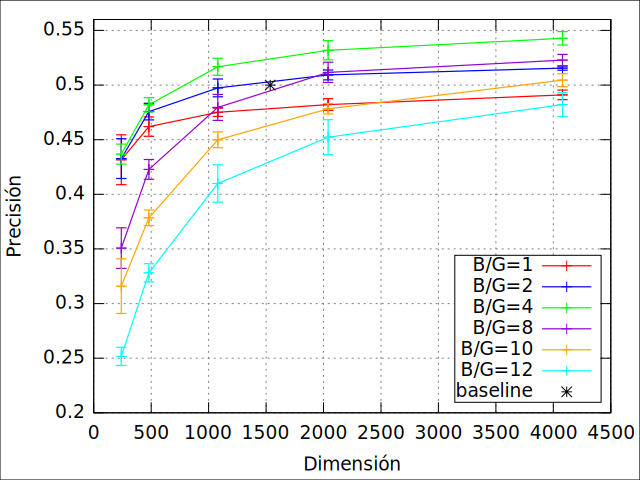
\includegraphics[width=8cm]{img/resultados/reales/mean.png}
				}
				\subfloat[Resultados usando la mediana \label{fig: Reales-mediana}]{
					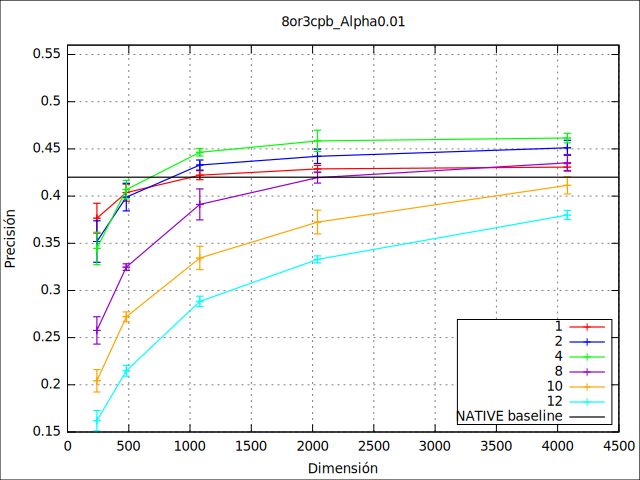
\includegraphics[width=8cm]{img/resultados/reales/median.png}
				}
				\\
				\subfloat[Resultados usando la distribución exponencial \label{fig: Reales-expon}]{
					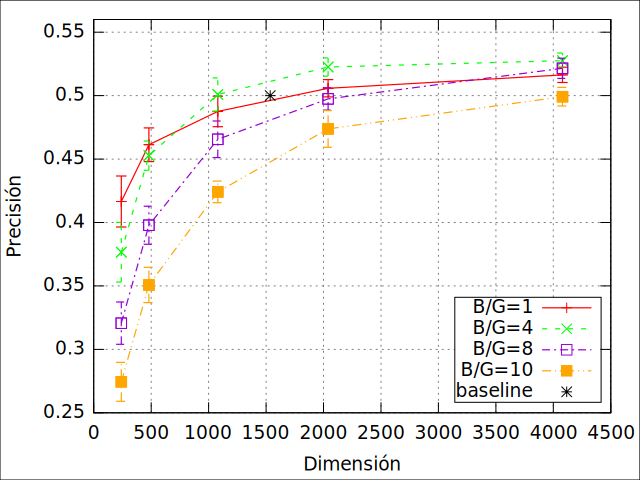
\includegraphics[width=8cm]{img/resultados/reales/expon.png}
				}
				\subfloat[Resultados usando bootstrap\label{fig: Reales-bootstrap}]{
					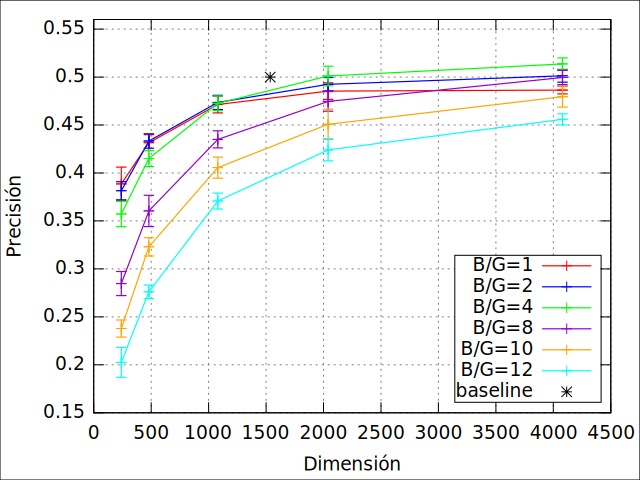
\includegraphics[width=8cm]{img/resultados/reales/bootstrap.png}
				}
				\caption[Resultados-Reales]{Esta figura presenta los resultados obtenidos por los 4 métodos propuestos para la binarización de los vectores.}
				\label{fig: Resultados-Reales}
			\end{figure}
			
	Teniendo en cuenta los resultados en \ref{fig: Resultados-Reales}, a simple vista se puede observar que los resultados obtenidos usando la media como método para binarizar los vectores son los mejores, llegando estos a un máximo cercano al $55\%$ de precisión. En el caso opuesto, el usar la mediana arrojó los peores resultados ya que en el mejor de los casos se supera el $47\%$ a diferencia de bootstrap que llega a $51\%$ . El uso de la distribución exponencial en los casos donde la longitud de los grupos es baja ($1$, $2$ bits por grupo) supera a la media en performance pero se mantiene por debajo a medida que aumentamos este valor (casos $\{ 4, 8, 10, 12\}$ bits por grupo). Los valores que podemos encontrar en \ref{fig: Reales-expon} se acercan a los del a media llegando a un máximo en la precisión de $53\%$. En cuanto al uso de bootstrap, se puede apreciar que los resultados se mantienen por debajo de los obtenidos con la distribución exponencial y la media con puntajes que rondan entre $45\%$ y $52\%$.
	
	En cuanto a las dimensiones evaluadas $\{ 240, 480, 1080, 2040, 4080 \}$ es claro que a medida que aumentamos la longitud de los vectores aumenta la performance. Se puede ver que, cuando se usan vectores de longitud reducida (en este caso $240$), se marca una diferencia importante en la precisión entre los experimentos realizados con grupos de dimensionalidad baja $\{ 1, 2, 4 \}$ y alta $\{8, 10, 12\}$. Es decir, dejando fija la dimensión de los vectores en $240$, mientras más chico es el tamaño de los grupos mejor es el resultado (se puede observar en cualquiera de los gráficos en \ref{fig: Resultados-Reales}). En el otro extremo, si usamos grupos de $12$ bits la precisión baja bastante. La misma relación se mantiene a medida que aumentamos el tamaño de los vectores de características hasta cierto punto. Por ejemplo, en \ref{fig: Resultados-Reales} y específicamente en \ref{fig: Reales-media} es claro que a partir del uso de $1080$ como tamaño de vector en adelante, el uso de grupos de longitud mayor arroja mejores resultados. Lo mismo sucede en las otras figuras en diferentes puntos. En cuanto al uso del valor $4080$, se puede ver que no hay un aumento considerable en la performance que lo diferencie del uso de $2040$. Con esto en mente, es conveniente hacer uso de este último valor ya que otorga resultados similares a los calculados con $4080$ usando vectores mucho más chicos incrementando la eficiencia en el cómputo.
	
	El problema con los vectores binarizados de dimensión reducida, es que almacenan menos información sobre la imagen a comparación de los vectores cuya longitud es mayor. Tal es el caso como se puede observar en \ref{fig: Resultados-Reales}. 
	
	Otro parámetro a analizar aquí es \textit{alpha} $\in \{ 0.0001, 0.001, 0.01, 0.1, 1\}$. Los mejores resultados de cada método se dieron cuando el valor de \textit{alpha} se estableció en $0.01$ y son los que se muestran en la figura \ref{fig: Resultados-Reales}. Valores por encima $0.01$ o muy cercanos a 0 no llegaron en los experimentos a igualar la precisión obtenida con el valor de \textit{alpha} elegido. Por cuestiones de espacio se decidió mostrar en esta sección los resultados que se obtuvieron con el mejor valor de \textit{alpha}. El resto de los gráficos se pueden encontrar en el apéndice ``B'' con el resto de los resultados de los experimentos. A medida que incrementamos el valor de \textit{alpha}, 
	
	Al igual que con el parámetro \textit{alpha}, hay $2$ parámetros que se dejaron fijos y son los relacionados con la función de HOG: la cantidad de \textit{orientaciones} y la cantidad de \textit{celdas por bloque}. Se decidió por usar $8$ y $9$ respectivamente ya que dichos valores devuelven los mejores resultados. 
	
			\begin{figure}[htbp]
				\centering
				\centerline{
					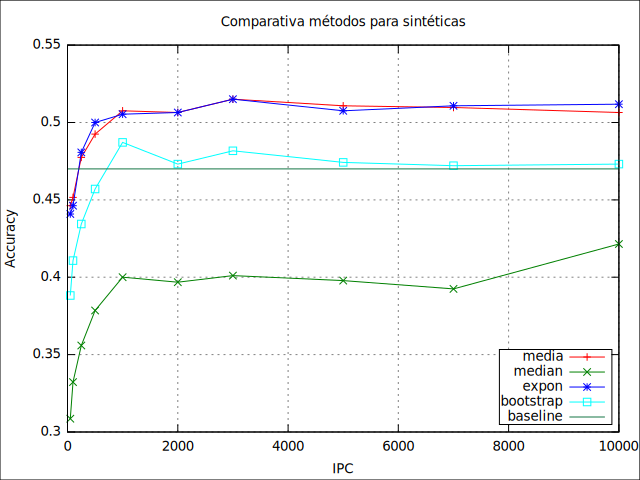
\includegraphics[scale=0.7]{img/resultados/reales/comparativa_metodos.png}
				}
				\caption[Reales comparativa]{El gráfico muestra las mejores curvas de los gráficos presentados en la figura \ref{fig: Resultados-Reales} con la mejor configuración}
				\label{fig: Reales-Comparativa metodos}
			\end{figure}
	
	Del análisis realizado surge que la mejor configuración está dada por \textit{alpha = $0.01$}, \textit{orientaciones = $8$}, \textit{celdas por bloque = $9$}, \textit{bits por grupo = $4$} y \textit{dimensión del vector = 4080}. Se puede observar en \ref{fig: Reales-Comparativa metodos} las mejores curvas para cada método utilizando la mejor configuración (a excepción de la longitud del vector con el objetivo de ver la curva de crecimiento). Queda claro que la media se puede establecer como el mejor método para la binarización por lo cual en los próximos experimentos se procederá a trabajar con el mismo. De la misma manera la mediana termina siendo el peor método. De este último caso se puede ver que incluso para la mejor configuración tiene a ``aplanarse'' a medida que aumentamos la dimensión del vector característica
		
	\begin{table}
		\centering
		\begin{tabular}{ | l | l | l | p{5cm} |}
    			\hline
    				\textbf{NATIVE + FERNS} & \textbf{Score} \\ \hline
    				Media & 0.54\% \\ \hline
    				Mediana & 0.47\%\\ \hline
    				Exponencial & 0.53\% \\ \hline
    				Bootstrap & 0.52\%\\ 
    			\hline
    		\end{tabular}
    		\caption[Resultados imagenes naturales]{Tabla comparativa entre los diferentes métodos propuestos para la binarización en la clasificación de caracteres en escenas naturales.}
    		\label{table: reales-comparativa}
    	\end{table}
    	
    	
    	\newpage
    	\subsubsection{Imágenes Sintéticas}
    	
    En esta etapa se procederán mostrar los resultados obtenidos de los experimentos con las imágenes sintéticas. Además, los gráficos van a representar la relación entre la cantidad de imágenes sintéticas por clase (dado por \textit{IPC} en las siguientes figuras) y la precisión de clasificación dada por los $6$ valores a evaluar que son las dimensiones de los grupos. Teniendo en cuenta los resultados anteriores con las imágenes reales, se decidió por trabajar $8$ orientaciones, $9$ celdas por bloque, alpha de $0.01$ y usando la media como método de binarización ya que son los parámetros que dieron los mejores resultados.
  
			\begin{figure}[htbp]
				\centering
				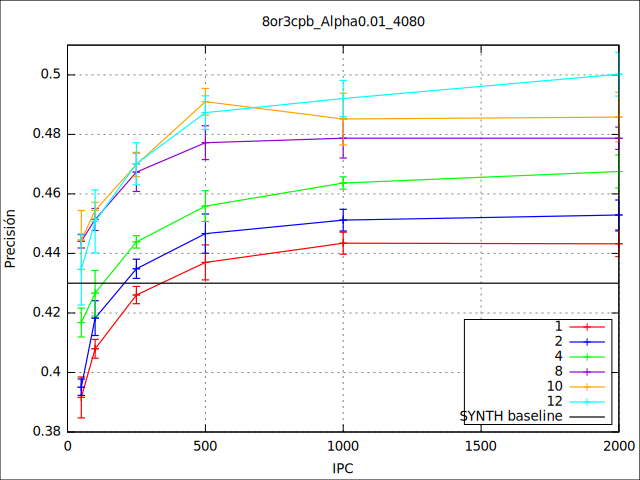
\includegraphics[scale=0.6]{img/resultados/sinteticas/mean_4080.png}
				\caption[Sintéticas media 4080]{El gráfico muestra los resultados obtenidos de haber utilizado la mejor configuración analizada y haciendo uso de vectores binarizados de longitud $4080$}
				\label{fig: Sinteticas-media-4080}
			\end{figure}

			\begin{figure}[htbp]
				\centering
				\includegraphics[scale=0.6]{img/resultados/sinteticas/mean_2040.png}
				\caption[Sintéticas media 2040]{EEl gráfico muestra los resultados obtenidos de haber utilizado la mejor configuración analizada y haciendo uso de vectores binarizados de longitud $2040$}
				\label{fig: Sinteticas-media-2040}
			\end{figure}
			
	Hacer texto con las siguientes ideas
	\begin{itemize}
		\item En los experimentos con imágenes sintéticas en general a más cantidad de imágenes por clase mayor es la performance de clasificación. Sin embargo llega un punto en que se deja de aumentar la perfomances y en varios casos disminuye despues de cierto punto.
		\item Es claro que para este tipo de experimentos es mejor tener grupos de dimensiones mayores a los propuestos para las imágenes reales. Analizar que los casos donde los grupos tienen 12 bits la performance decae a comparación de los casos donde los mismo tienen 10 bits.
		\item Defenitivamente la mediana y bootstrap no son buenos métodos para binarizar.
	\end{itemize}
			
\newpage
    	\subsubsection{Imágenes Reales y Sintéticas}
    	
	Por último se van a mostrar los resultados correspondientes de haber entrenado al clasificador con conjuntos de entrenamiento mixtos. Se procederá a mostrar los gráficos con las mejores y peores configuraciones y sus resultados. También se mostrarán las matrices de correlación para todos estos casos. Teniendo en cuenta el análsis anterior, se van a mostrar los resultados de haber utilizado solamente la la media como umbral ya que fue la que retornó los mejores valores.
	
	El gráfico a continuación presenta el eje \textit{x} en escala logarítmica para poder apreciar mejor las variaciones que se dan al experimentar con valores cercanos entre sí.
	
			\begin{figure}[!htbp]
				\centering
				\includegraphics[scale=0.6]{img/resultados/mixtas/best_mean.png}
				\caption[Mixtas media mejor resultado]{El gráfico muestra la configuración que devolvió los mejores resultados.}
				\label{fig: Mixtas-media-mejor}
			\end{figure}

	De la figura \ref{fig: Mixtas-media-mejor} se puede desprender el siguiente análisis. El primero, y uno de los más importantes, hace referencia a la influencia en la clasificación de ir agregando de manera incremental imágenes sintéticas durante la etapa de entrenamiento. Se puede observar que a nivel general todos los experimentos llegaron a un punto donde su performance se desplomó al seguir agregando imágenes sintéticas en el entrenamiento. Sin embargo, este cambio ocurrio en diferentes momentos dependiendo del caso. Por ejemplo, cuando trabajamos con grupos de dimensionalidad baja ($1$, $2$ y $4$ bits por grupo), la precisión del clasificador va en aumento hasta que se llega a un máximo correspondiente al haber entrenado al sistema con igual cantidad de imagenes reales y sintéticas. A partir de ese punto el seguir incrementando la proporción de sintéticas sobre reales trajo efectos negativos en los resultados como se puede apreciar en el gráfico presentado. En los casos donde consideramos $10$ y $12$ bits por grupo el rendimiento se desploma cuando consideramos más de 75 imágenes sintéticas. La mejor curva en el gráfico la obtenemos cuando consideramos $8$ bits por grupo y entrenamos al clasificador con el doble de imágenes sintéticas que reales. Este resultado difiere con respecto al análisis realizado para los experimentos con imágenes reales donde consideramos que el mejor parámetro era considerar grupos de $4$ bits. En la mayoría de los casos se dan buenos resultados cuando la cantidad de imágenes sintéticas sobre las reales es la misma ($1$, $2$ y $4$) o se duplica ($8$ y $10$).
	
	Una de las diferencias con los análisis realizados en los experimentos con imágenes reales, es que el mejor resultado se encuentra cuando se usan grupos de $8$ bits. 


			\begin{figure}[!htbp]
				\centerline{\includegraphics[scale=0.4]{img/resultados/mixtas/best_mean_matrix_Alpha0,01_4080-8.png}}
				\caption[Mixtas Matriz expon]{Matriz de correlación del gráfico \ref{fig: Mixtas-media-mejor} para el mejor resultado. \RC{Demasiado grande las matrices como para mostrarlas y que se vean bien}}
				\label{fig: Mixtas-Matrix-media-mejor}
			\end{figure}
	
			\begin{figure}[!htbp]
				\centerline{\includegraphics[scale=0.4]{img/resultados/mixtas/best_mean_matrix_Alpha0,01_4080-8_ins.png}}
				\caption[Matriz de correlación ``case insensitive'' para mixtas media]{Matriz de correlación del gráfico \ref{fig: Mixtas-media-mejor} para el mejor resultado no teniendo en cuenta los caracteres en mayúscula.}
				\label{fig: MatrizIns-Mixtas-media-mejor}
			\end{figure}



	\newpage
\subsection{Análisis}
	Análisis / discusión
	\begin{itemize}
		\item Comparar la performance al usar diferentes datasets (comparar cantidad de imágenes por clase al usar caracteres sintéticos). Hacer una tabla.
		\item Observaciones sobre errores de clasificación. El problema que surge con algunos caracteres donde no se puede distinguir minúscula de mayúscula con lo cual se producen errores. Mostrar la matriz de confusión del mejor caso donde no se distingan mayúsculas de minúsculas. Otro error donde ciertos caracteres como la "l" se confunden con otros caracteres como el "1".
		\item Comparar en los resultados con los obtenidos por Wang et al. en condiciones similares. Básicamente explicar algo que no explican en su trabajo Wang et al. y que es la influencia en la cantidad de muestras sintéticas por clase.
		\item Análisis de como aumenta la performance de clasificación el mezclar imágenes sintéticas y reales. Mostrar como a medida que aumentamos demasiado la proporción de img. sintéticas, se tiende a disminuir la precisión. Básicamente, la precisión baja para "igualarse" a la precisión obtenida cuando se entrena al clasif con puras imagenes sintéticas (usando la misma cant. de img. por clase).
	\end{itemize}


	%\subsection{Implementación}

	\begin{itemize}
		\item Explicar porque uso python + las librerías involucradas.
		\item Porque uso JSON y no MySQL para almacenar datos.
		\item Datasets usados y su creación.
		\item Pipeline implementado desde la creación del dataset hasta la obtención de resultados del clasificador Random Ferns.
	\end{itemize}

	


	
	\newpage
\section{Conclusiones y trabajos futuros}

	Para concluir con este trabajo y en base a los resultados expuestos, se puede destacar que el trabajo de reconocimiento de caracteres en imágenes estructuradas no es una tarea sencilla. Actualmente han habido bastantes avances en el campo pero todavía no  se logra desarrollar un método que compita con los clasificadores que hacen reconocimiento de texto impreso.
	
	Basados en los análisis del capítulo 4, se pudo observar que el uso de imágenes sintéticas proporcionó mejoras al momento de entrenar al clasificador si se las combina con imágenes reales. Si bien la mejora no es muy notoria, se puede seguir trabajando para mejorar esto y así poder evitar a futuro el tedioso trabajo de tener que recolectar imágenes reales. Una mejora interesante para agregar en la generación de imágenes sintéticas es tener un conjunto de fondos naturales para poder usar o darle color a los caracteres. Si bien todas las imágenes terminan en escala de grises, las pequeñas variaciones que se introducen al agregar estos detalles pueden ayudar a mejorar la clasificación.
	
	El uso de Random Ferns como clasificador es una buena opción por lo expuesto en el capítulo 2; sin embargo, sería interesante probar con otros clasificadores para poder realizar una mejor comparación.
	
	Sin duda alguna el desafio de reconocer texto en escenas naturales es un problema que vale la pena estudiar y pulir ya que las aplicaciones que tiene actualmente son enormes. Más aún con la proliferación de los dispositivos móviles y la necesidad de crear aplicaciones que asistan a usuarios con deficiencia visual entre otros.

	\newpage	
\addcontentsline{toc}{section}{Referencias}		% sino no figura en el TOC

\begin{thebibliography}{100}

	\bibitem{wang}
 	 	Kai Wang, Boris Babenko and Serge Belongie,
	 	\emph{``End-to-End Scene Text Recognition''},
		IEEE International Conference on Computer Vision (ICCV), 
		Barcelona, España,
		2011.
		
	\bibitem{WB10}
 	 	Kai Wang and Serge Belongie,
	 	\emph{``Word spotting in the wild''},
		In ECCV, 2010.
		
	\bibitem{fischler}
 	 	M.A. Fischler and R.A. Elschlager,
	 	\emph{``The representation and matching of pictorial
structures''},
		IEEE Transactions on Computer, 
		22(1):67–92,
		Enero 1973.
		
	\bibitem{Bis07}
		Christopher M. Bishop.
		\emph{``Pattern Recognition and Machine Learning (Information Science and Statistics)''}.
		Springer, Octubre 2007.
		
	\bibitem{dCBV09}
		T. E. de Campos, B. R. Babu, and M. Varma.
		Character recognition in natural images.
		In \emph{``Proceedings of the International Conference on Computer Vision Theory and Applications, Lisbon, Portugal,''}
		February, 2009.
		
	\bibitem{KGK^{+}07}
		Sunil Kumar, Rajat Gupta, Nitin Khanna, Santanu Chaudhury, and Shiv Dutt Joshi.
		\emph{``Text extraction and document image segmentation using matched wavelets and mrf model.''}
		\textit{IEEE Transactions on Image Processing}, 16(8):2117-2128, 2007.
	
	\bibitem{DT05}
		Navneet Dalal \& Bill Triggs.
		\emph{``Histograms of oriented gradients for human detection.''}
		In Cordelia Schmid, Stefano Soatto, and Carlo Tomasi, editors, \textit{International Conference on Computer Vision \& Pattern Recognition}, volume 2, pages 886-893, INRIA Rh\^{o}ne-Alpes, ZIRST-655, av. de l'Europe, Montbonnot-38334, June 2005.
		
	\bibitem{PSH2011}
		J. Pradeep, E. Shrinivasan \& S. Himavathi,
		\emph{``Diagonal Based Feature Extraction for Handwritten Alphabets Recognition System Using Neural Network''},
		International Journal of Computer Science \& Information Technology(IJCSIT),
		vol.3, No 1, February 2011.
		
	\bibitem{Suen86}
		C. Y. Suen,
		\emph{``Character recognition by computer and applications''},
		in Handbook of Patter Recognition and Image Processing,
		New York: Academic,
		pp. 569-586,
		1986

	
	%\bibitem{RVJA2012}
	%	R. Verma \& J. Ali,
	%	\emph{``A-Survey of Feature Extraction and Classification Techniques in OCR Systems''},
	%	International Journal of Computer Applications \& Information Technology,
	%	Vol. I, Issue III,
	%	November 2012 (ISSN: 2278-7720).
		
	\bibitem{Heutte98}
		L. Heutte, T. Paquet, J. V. Moreau, Y. Lecourtier and C. Olivier,
		\emph{``Structural/statistical feature based vector for handwritten character recognition''},
		Pattern Recognition Letters,
		Vol. 19(7), pp. 629-641,
		1998.
		
	\bibitem{Hussain72}
		A. B. S. Hussain, G. T. Toussaint and R. W. Donaldson,
		\emph{``Results obtained using a simple character recognition procedure on Munson’s handprinted data''},
		IEEE Transactions on Computers, pp. 201-205,
		1972.
		
	\bibitem{Glauberman56}
		M. H. Glauberman,
		\emph{``Character recognition for business
machines''},
		Electronics,
		Vol. 29, pp. 132-136,
		1956.
		
	\bibitem{TR93}
		R. Tarling and R. Rohwer,
		\emph{``Efficient use of training data in
the n-tuple recognition method''},
		Electronics Letters,
		Vol. 29(24), pp. 2093-2094,
		1993
		
	\bibitem{RP94}
		J. Rocha and T. Pavlidis,
		\emph{``A shape analysis model with applications to a character recognition system''},
		IEEE Transactions on PAMI,
		Vol. 16(4), pp. 393-404, 
		1994.
		
	\bibitem{Amin2000}
		A. Amin,
		\emph{``Recognition of printed Arabic text based on global features and decision tree learning techniques''},
		\textit{Patter Recognition},
		Vol. 33, pp. 1309-1323,
		2000.
	
	\bibitem{NNSJ}
		Nadira Muda, Nik Kamariah, Nik Ismail, Siti Azami Abu Bakar, Jasni Mohamad Zain,
		\emph{``Optical Character Recognition By Using Template Matching(Alphabet)''},
		Universiti Malaysia Pahang.
		
	\bibitem{SA96}
		S. Lucas, A. Amiri
		\emph{``Statistical Syntactic Methods for High Performance OCR''}
		Vision, Image and Signal Processing, IEE Proccedings,
		vol. 134, Issue 1, pp. 23-30,
		February 1996.
		
	\bibitem{RYVY2010}
		Raghuraj Singh, C. S. Yadav, Prabhat Verma, Vibhash Yadav,
		\emph{``Optical Character Recognition (OCR) for Printed Devnagari Script Using Artificial Neural Network''},
		International Journal of Computer Science \& Communication,
		January-June  2010.
	
	\bibitem{Eikvil}
		Line Eikvil.
		\emph{``Optical Character Recognition''}.
		\url{http://www.nr.no/~eikvil/OCR.pdf}.
		December, 1993.
		
	\bibitem{GKurt}
		Dr. Gordon Kurtenbach (2010).
		\emph{``Pen-Based Computing''}.
		\emph{XRDS}, vol.16, num.4, pp.14-20.
		Obtenido de \url{http://www.autodeskresearch.com/pdf/penbasedcomputing-kurtenbach.pdf}.
		
	\bibitem{x-root}
		Andor Grei{\ss}l.(2009).
		\emph{Cardreader}(v2.0.10)[Mobile Application Software].
		Obtenido de \url{https://itunes.apple.com/de/app/id333992036?mt=8}
		
	\bibitem{arh-anpr}
		ARH Inc.
		\emph{The CARMEN\textregistered Parking ANPR Software}[Computer Software].
		Obtenido de \url{http://www.anpr.net/anpr_09/anpr_parking.html}
		
	\bibitem{arh-passport}
		ARH Inc.
		\emph{PRM(Passport Reader Multireader)}[Computer Device].
		Obtenido de \url{http://www.passport-reader.com/prm_passport_reader.html}
		
	\bibitem{arh-card}
		ARH Inc.
		\emph{Card Reader}[Computer Device].
		Obtenido de \url{http://www.passport-reader.com/card_reader.html}
	
	\bibitem{creaceed}
		Creaceed S.P.R.L (2010).
		\emph{Prizmo}(v3.1.5)[Mobile Application Software].
		Obtenido de \url{https://itunes.apple.com/gb/app/prizmo-scanning-ocr-speech/id366791896?mt=8}
		
	\bibitem{sunnyside}
		SUNNYSIDESOFT (2013).
		\emph{VirtualTablet Lite (S-Pen)}(v1.2)[Mobile Application Software].
		Obtenido de \url{https://play.google.com/store/apps/details?id=com.sunnysidesoft.VirtualTablet}
		
	\bibitem{gbook}
		Google Inc.(2004).
		\emph{Google Books}[Web Service].
		Obtenido de \url{http://books.google.com/}.
		
	\bibitem{Tauschek}
		G. Tauschek,
		\emph{``Reading Machine''},
		U.S. Patent 2026329,
		December 1935.
		
	\bibitem{Handel}
		P. W. Handel,
		\emph{``Statistical machine''}
		U.S. Patent 1915993,
		June 1933.
	
	\bibitem{Tesseract}
		Google Inc.(2005).
		\emph{``Tesseract''}
		Obtenido de \url{https://code.google.com/p/tesseract-ocr/}
		
	\bibitem{YoutubeStats}
	Google Inc.
	\emph{``Youtube statistics''}.
	Obtenido de \url{http://www.youtube.com/yt/press/es/statistics.html}
	
	\bibitem{Websites}
	Google Inc. 
	Official Blog.
	Obtenido de \url{http://googleblog.blogspot.com.ar/2008/07/we-knew-web-was-big.html}
	
	\bibitem{GoogleSearches}
	Statistic Brain.
	\emph{``Google Annual Search Statistics''}(2014).
	Obtenido de \url{http://www.statisticbrain.com/google-searches/}
	
	\bibitem{DP97}
		Domingos, P. y M. Pazzani (1997).
		\emph{``On the optimality of the simple bayesian classifier under zero-one loss''}. \textit{Machine Learning} 29, pp. 103-130.
		
	\bibitem{SpamPaper}
		T. S. Guzella, W. M. Caminhas.
		\emph{A review of machine learning approaches to Spam filtering}.
		Expert Systems with Applications.
		2009.
		
	\bibitem{BrownLowe07}
		Brown, M. and Lowe, D. (2007).
		\emph{``Automatic panoramic image stitching using invariant features''}.
		\textit{International Journal of Computer Vision},
		74(1):59–73.
	
	\bibitem{FPZ07}
		Fergus, R., Perona, P., and Zisserman, A. (2007).
		\emph{``Weakly supervised scale-invariant learning of models for visual recognition''}.
		\textit{International Journal of Computer Vision},
		71(3):273–303.
		
	\bibitem{Breiman01}
		Breiman, L.
		\emph{``Random Forests''}.
		Machine Learning 45(1), 5-32.
		January 2001.
		
				
	\bibitem{HOGImages}
		Levi G., (2013, August 18).
		\emph{``A Short introduction to descriptors''}[blog post].
		Obtenido de \url{http://gilscvblog.wordpress.com/2013/08/18/a-short-introduction-to-descriptors/}.
	
	\bibitem{Ozuysal}
		Ozuysal, M., Calonder, M., Lepetit, V. \& Fua, P.
		\emph{``Fast Keypoint Recognition using Random Ferns''}.
		IEEE Transactions on Pattern Analysis and Machine Intelligence,
		32, 448-461 (2010)
		
	\bibitem{DAB}
		Donoser, M., Arth, C. \& Bischof, H.
		\emph{``Detecting, Tracking and Recognizing License Plates''}.
		Institute for Computer Graphic and Vision.
		
	\bibitem{Nadejda}
		Nadejda S. Roubtsova , Rob G.J. Wijnhoven and Peter H.N. de With.
		\emph{``Integrated Text Detection and Recognition in Natural Images''}.
		
	\bibitem{LoweDavid04}
		Lowe, David G. (2004).
		\emph{``Distinctive Image Features from Scale-Invariant Keypoints''}.
		\textit{International Journal of Computer Vision.}
		
	\bibitem{LoweDavid99}
		Lowe, David G. (1999).
		\emph{``Object recognition from local scale-invariant features''}.
		Proceedings of the International Conference on Computer Vision 2.
		pp. 1150–1157.
		
	\bibitem{SJC08}
		J. Shotton, M. Johnson, and R. Cipolla.
		\emph{``Semantic texton forests for image categorization and segmentation''}.
		In \textit{CVPR}, 2008.
		
	\bibitem{OFL07}
		M. Ozuysal, P. Fua, and V. Lepetit.
		\emph{``Fast keypoint recognition in ten lines of code''}.
		In \textit{CVPR}, 2007.
		
	\bibitem{QuinlanID3}
		J. R. Quinlan.
		\emph{Induction of Decision Trees}.
		Machine Learning 1: 81-106.
		March 1986.
		
	\bibitem{QuinlanC45}
		J. R. Quinlan.
		\emph{C4.5: Programs for Machine Learning}.
		Morgan Kaufmann Publishers, 1993.
		
	\bibitem{PDomingo}
		P. Domingo.
		\emph{``A Few Useful Things to Know about Machine Learning''}.
		Department of Computer Science and Engineering.
		University of Washington.
		
	\bibitem{GPP03}
		B. Gatos, I. Pratikakis and S. Perantonis.
		\emph{``Towards Text Recognition in Natural Scene Images''}.
		Computational Intelligence Laboratory, Institute of Informatics and Telecommunications.
		
	\bibitem{LNJM}
		L. Neumann and J. Matas.
		\emph{``Real-Time Scene Text Localization and Recognition''}.
		In \textit{CVPR}, 2012.
		
	\bibitem{PiotrD}
		Piotr Dollár.
		\emph{Piotr's Image and Video Matlab Toolbox (PMT)}.
		Obtenido de \url{http://vision.ucsd.edu/~pdollar/toolbox/doc/index.html}. 
		
	\bibitem{LBreiman96}
		L. Breiman.
		\emph{Bagging Predictors}.
		Septiembre 1994.
		
		
		
				
\end{thebibliography}
	
	%\newpage	
\appendix
\subsubsection{Conceptos de probabilidad y notación}
	\RC{Reformular todo}
	A continuación se introducirán algunos conceptos de probabilidad, que serán de utilidad en el desarrollo de las secciones posteriores.

	\paragraph*{Variables aleatorias discretas} ~\\

		La expresión $p(A)$ denota la probabilidad de que el evento $A$ sea verdadero. Por ejemplo, $A$ puede ser la expresión lógica ``Va a llover mañana''. Se requiere que $0 \leq p(A) \leq 1$, donde $p(A)=0$ significa que el evento no va a ocurrir, y $p(A)=1$ significa que el evento definitivamente va a suceder. Escribimos $p(\overline{A})$ para denotar la probabilidad del evento no $A$, es decir, de que el evento no ocurra; esto se define como $p(\overline{A})=1-p(A)$. Se escribirá $A=1$ para hacer referencia que el evento $A$ es verdadero, y $A=0$ cuando el evento $A$ es falso.
		
		Se puede extender la noción de eventos binarios definiendo una \textit{variable aleatoria discreta} $X$, la cual puede tomar cualquier valor de un conjunto finito o infinito contable \scalebox{1.4}{$\chi$}. Se denota la probabilidad de que $X=x$ por $p(X=x)$, o sólo $p(x)$ como abreviación, ambas notaciones se van a usar indistintamente en el desarrollo del trabajo. Aquí $p()$ se denomina \textit{función de probabilidad}. Esta satisface las propiedades $0 \leq p(x) \leq 1$ y $\sum_{x \in \chi}p(x)=1$.
		
	\paragraph*{Probabilidad de la unión de dos eventos} ~\\
		
		Dados dos eventos, $A$ y $B$, se define la probabilidad de A o B de la siguiente manera:
		\begin{align}
			p(A \lor B) &= p(A) + p(B) - p(A \land B) \\
			&= p(A) + p(B) ~\text{si A y B son mutuamente excluyentes}
		\end{align}
		
	\paragraph*{Probabilidad conjunta} ~\\
	
		Se define la probabilidad del evento conjunto A y B como sigue:
		\begin{align}
			p(A,B) = p(A \land B) = p(A|B)p(B)
		\end{align}

		A esta ecuación se la llama \textit{regla del producto}. Dada la distribución conjunta en dos eventos p(A,B), se define la ``distribución marginal'' de la variable aleatoria $A$ de la siguiente manera:
		\begin{align}
			p(A)=\sum_{b}p(A|B=b)p(B=b)
		\end{align}
		donde se asumen todos los estados posibles de B. Se puede definir p(B) de forma similar. A esta ecuación se la denomina regla de la suma o la regla de la probabilidad total.
		
	\paragraph*{Probabilidad condicional} ~\\
	
		Se define la probabilidad condicional del evento A, dado que el evento B es verdadero, como sigue:
		\begin{align}
			p(A|B) = \frac{p(A,B)}{p(B)} ~\text{si}~ p(B)>0
		\end{align}
		
	\paragraph*{Regla de Bayes} ~\\
		
		Combinando la definición de probabilidad condicional con las reglas del producto y la suma se obtiene la \textit{regla de Bayes}, también llamada \textit{Teorema de Bayes}:
		\begin{align}\label{eq:bayes}
			p(X=x|Y=y) &= \frac{p(X=x,Y=y)}{p(Y=y)} \\
			&= \frac{p(X=x)p(Y=y|X=x)}{\sum_{x'}p(X=x')p(Y=y|X=x')}
		\end{align}

	\paragraph*{Independencia e independencia condicional} ~\\
	
		Se dice que $X$ e $Y$ son \textit{incondicionalmente independientes} o \textit{marginalmente independientes}, denotado como $X \bot Y$	, si se puede representar la unión como el producto de dos marginales, es decir,
	\begin{align}
		X \bot Y \Longleftrightarrow p(X,Y) = p(X)p(Y)
	\end{align}			
			
		En general, se dice que un conjunto de variables es mutuamente independiente si la unión puede ser escrita como producto de marginales.
		
		Desafortunadamente, la independencia incondicional es rara, porque la mayoría de las variables pueden influir en la mayoría de las otras variables. Sin embargo, usualmente esta influencia se da a través de otras variables en vez de ser directa. Por lo tanto se dice que $X$ e $Y$ son \textit{condicionalmente independientes} dada $Z$ si y solo si la unión condicional puede ser escrita como producto de marginales condicionales:
		\begin{align}
			X \bot Y|Z \Longleftrightarrow p(X,Y|Z) = p(X|Z)p(Y|Z)
		\end{align}
	



	%\newpage
Córdoba, Argentina, 2014\\[9.5cm]
\begin{flushright}
    \textit{Rodrigo Carranza Astrada}
\end{flushright}

	
\end{document}
